\documentclass{jsarticle}

\usepackage[dvipdfmx]{graphicx}
\usepackage{float} %図を指定の位置に置
\usepackage{moreverb}

\begin{document}
 
\begin{center}
\vspace*{1cm}
\large
{\LARGE 卒業研究報告書}\\
\vspace*{0.8cm}
題目\\
\vspace*{1cm}
{\Huge \underline{プロセスマイニングを用いた} \\ \underline{店舗に並ぶ行列の分析}}
\vspace{3mm}
 
\vspace*{3cm}
指導教員\\
\vspace*{0.3cm}
\underline{\LARGE 森山 真光 准教授}\\
%\vspace*{-0.3cm}
%\underline{\hspace*{5cm}}\\
\vspace*{3cm}
報告者\\
\vspace*{0.3cm}
 
{19--1--037--0177}\\
\vspace*{0.3cm}
\underline{\Huge 李 晃史}\\
% \vspace*{-0.3cm}
% \underline{\hspace*{5cm}}\\
\vspace*{0.5cm}
近畿大学理工学部情報学科\\
\vspace*{2cm}
提出日:\today 
\end{center}




\newpage
\begin{abstract}
近年、コロナ禍により飲食店におけるテイクアウトの需要が高まっている。
そんな中、店舗販売と併用してモバイルオーダーでのテイクアウト注文を導入した店舗で、
モバイルオーダーでのテイクアウト注文を無制限に受け入れ過ぎたことによって
店舗が混雑し販売に支障をきたす事態や、逆に注文の受け入れ制限をしたことにより
早く注文を処理できた場合に本来受け入れることができた注文分の利益を損失する事態が起きている。
そこで、適切な受け入れ人数を設定するために行列分析を目的とし店舗の行列の計測を行いプロセス マイニングを用いて行列の分析をした。

行列データの収集方法を示し、ExpoGoを用いて近大ラーメンにて行列の計測を行った。
7月の行列計測は行列参加時間、注文開始時間、決済開始時間、注文完了時間、商品受け取り時間の
5つの区分に分けて計測した。
12月の行列計測は7月に計測した上記の5つの区分に加えて、
新たに性別とグループ人数の項目も追加して計測を行った。
行列データをプロセスマイニングを用いてフィルタリング等を行い、
プロセスマップを作成し分析を行った。

5日間の行列計測を行ったが、行列時間や商品受取待ち時間は来店数が増加するに連れ
長くなる傾向がみられた。それを示すデータとして、行列時間は12/16を除いて混雑時の方が待ち時間が長くなっており、商品受取待ち時間は計測日全てにおいて混雑時の方が待ち時間が長くなっていた。
性別やグループ人数別での分析では、ある一定の傾向はみられなかった。
性別の区分における注文時間や決済時間よりもグループの区分における注文時間や決済時間の方が大きく時間差が生じたことが分かった。
これは、友達同士や複数人で券売機を前にすると、同時購入による時間短縮や、券売機前でのメニューの相談による時間遅延が生じたからであると言える。
性別の区分ではあまり差が生じず、グループ人数別ではバラツキが生じやすく一定の傾向はないと考えられる。






 
\end{abstract}





\newpage
\normalsize

%\maketitle
\tableofcontents





\newpage  
\section{序論}
\subsection{本研究の背景}
近年、コロナ禍により飲食店におけるテイクアウトの需要が高まっている。
飲食店においてテイクアウトの需要が高まっている事を示すデータがある。
株式会社プレシャスパートナーズが行なった931の飲食店から得た年末の営業に関しての
調査\footnote{5割以上の飲食店が新型コロナウイルスの影響でテイクアウトを開始/931名に聞いた飲食店の年末の営業と採用活動に関する調査 https://www.foods-ch.com/news/prt\_76113/}
では、図\ref{fig:1}よりテイクアウトを行なっていると回答したのが68.5\%、
図\ref{fig:2}よりその中で新型コロナウイルスの影響でテイクアウトを始めたと
回答したのが54.7\%と半数以上になる。
また、株式会社ランプが全国の20代〜50代の男女889名を対象に行ったテイクアウトの利用実態
調査\footnote{テイクアウトの利用実態調査を実施。コロナ禍の外出自粛によりテイクアウトの利用頻度が増加した人は約6割。事前予約を希望する人が84.4\%の結果に。https://prtimes.jp/main/html/rd/p/000000020.000033995.html}では、
図\ref{fig:6}より新型コロナウイルスの影響でテイクアウトの事前予約・決済を希望する人は
84.4\%にものぼる。
この結果からモバイルオーダーを利用したテイクアウトの需要は高まっていることが確認できる。

そんな中、店舗販売と併用してモバイルオーダーでのテイクアウト注文を導入した店舗で、
モバイルオーダーでのテイクアウト注文を無制限に受け入れ過ぎたことによって店舗が混雑し
販売に支障をきたす事態\cite{bibi1}や、逆に注文の受け入れ制限をしたことにより早く注文を処理できた場合に
本来受け入れることができた注文分の利益を損失する事態が起きている。
従ってモバイルオーダーでのテイクアウト注文を無制限に受け入れるのではなく、
利用率がある一定の値を越えないように注文の受け入れ制限をすることで、
店舗での混雑による支障や利益損失を防ぐことができるのではないかと考えられる。

\begin{figure}[H]
  \centering
  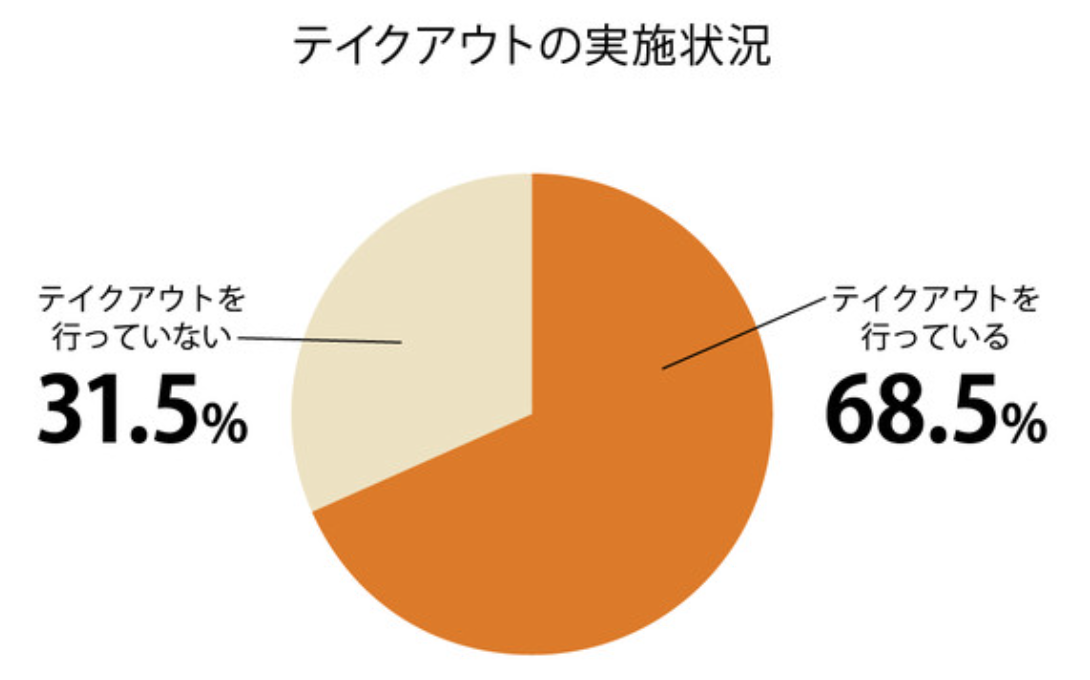
\includegraphics[width=10cm]{1.png}
  \caption{テイクアウトの実施状況}
  \scriptsize(出典:931の飲食店から得た年末の営業に関しての調査.株式会社プレシャスパートナーズ.)
  \label{fig:1}
\end{figure}

\begin{figure}[H]
  \centering
  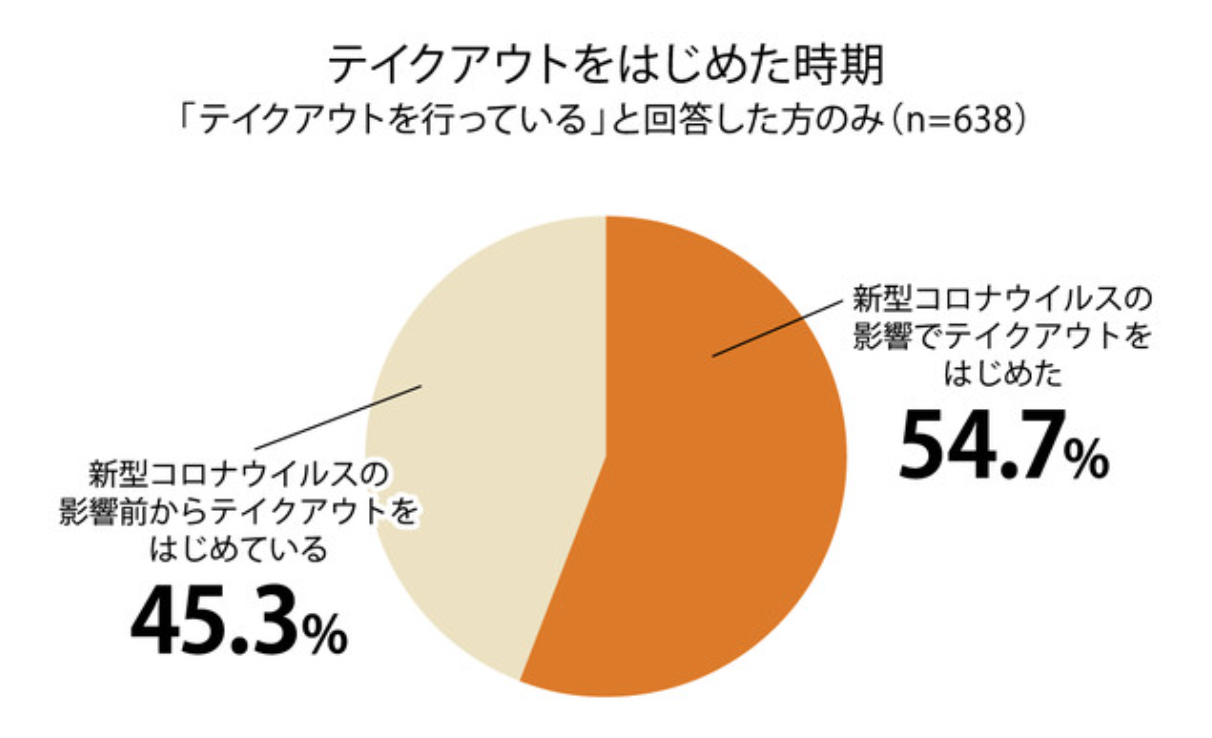
\includegraphics[width=10cm]{2.png}
  \caption{テイクアウトを始めた時期}
  \scriptsize(出典:931の飲食店から得た年末の営業に関しての調査.株式会社プレシャスパートナーズ.)
  \label{fig:2}
\end{figure}

\begin{figure}[H]
  \centering
  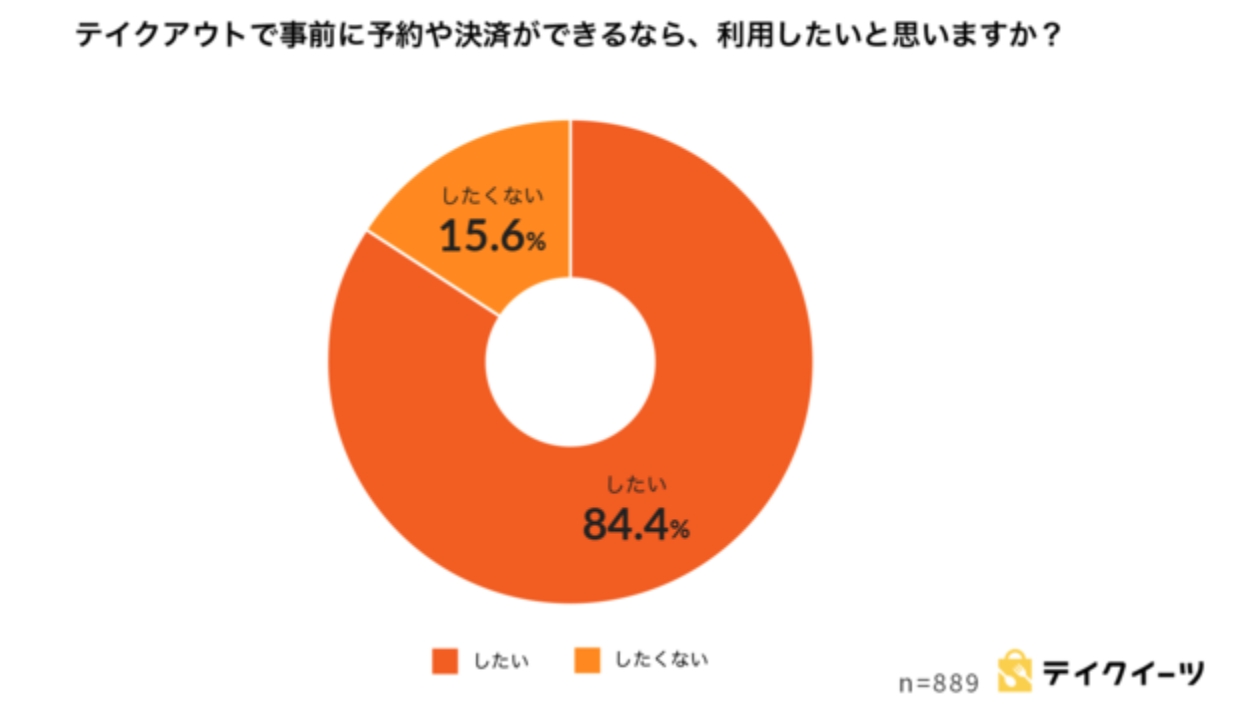
\includegraphics[width=10cm]{6.png}
  \caption{テイクアウト注文の事前予約・決済を希望する人}
  \scriptsize(出典:テイクアウトの利用実態調査.株式会社ランプ.)
  \label{fig:6}
\end{figure}








\newpage
\subsection{本研究の目的}
店舗販売と併用してモバイルオーダーでのテイクアウト注文の受け入れ人数を無制限や適当に設定すると、店舗の混雑や利益損失を起こす可能性がある。
モバイルオーダーでのテイクアウト注文を無制限に受け入れるのではなく、
利用率がある一定の値を越えないように注文の受け入れ制限をすることで、
店舗での混雑による支障や利益損失を防ぐことができるのではないかと考えられる。
適切な受け入れ人数を設定するためにはまず優先的に行列の特徴を知る必要があるので、
本研究では行列分析を目的とし店舗の行列の計測を行いプロセスマイニングを用いて行列の分析を行う。
店舗での行列計測については、近畿大学東大阪キャンパスにある近大をすすらんか様に承諾を得て行う。



\subsection{本報告書の構成}
2章では本研究を進めるにあたり調査した関連技術と関連研究を示す。
3章では行列データの収集方法と行列データの分析計画を示す。
4章では計測したデータの分析と考察を示す。
5章では結論及び今後の課題について示す。




\newpage


\section{関連技術・研究}
\subsection{プロセスマイニング}
プロセスマイニングとは、従業員が操作する各種業務システムのイベントログに基づく
ビジネスプロセスを分析することで業務プロセスを自動的に可視化し、
問題箇所を特定する分析手法である。プロセス管理の分野における一連の技術である。
プロセスマイニングは、大企業などで商品購入までのプロセス改善などに導入されている。
記録されたイベントログに含まれる傾向、パターン等の詳細を識別するために
イベントログに特殊なデータマイニングアルゴリズムを適用する。
プロセスマイニングを用いた分析からは除去しても支障のない「無駄な業務」や、
処理待ちが発生しやすくイベント全体の時間を長引かせてしまっている
「ボトルネック」などの問題を発見できる。
また、各イベントを行うのにかかった時間や平均時間を抽出し、
一定の時間間隔でのデータやグラフを得ることができる。

本研究では、プロセスマイニングのツールとしてApromoreを使用する。
図\ref{fig:3}はApromoreの分析画面であり、中央にはプロセスマップが表示されている。
ピンク色のノードは各アクティビティとなっていて、矢印の上の時間は、アクティビティから次のアクティビティにかかった時間を表している。

\begin{figure}[H]
  \centering
  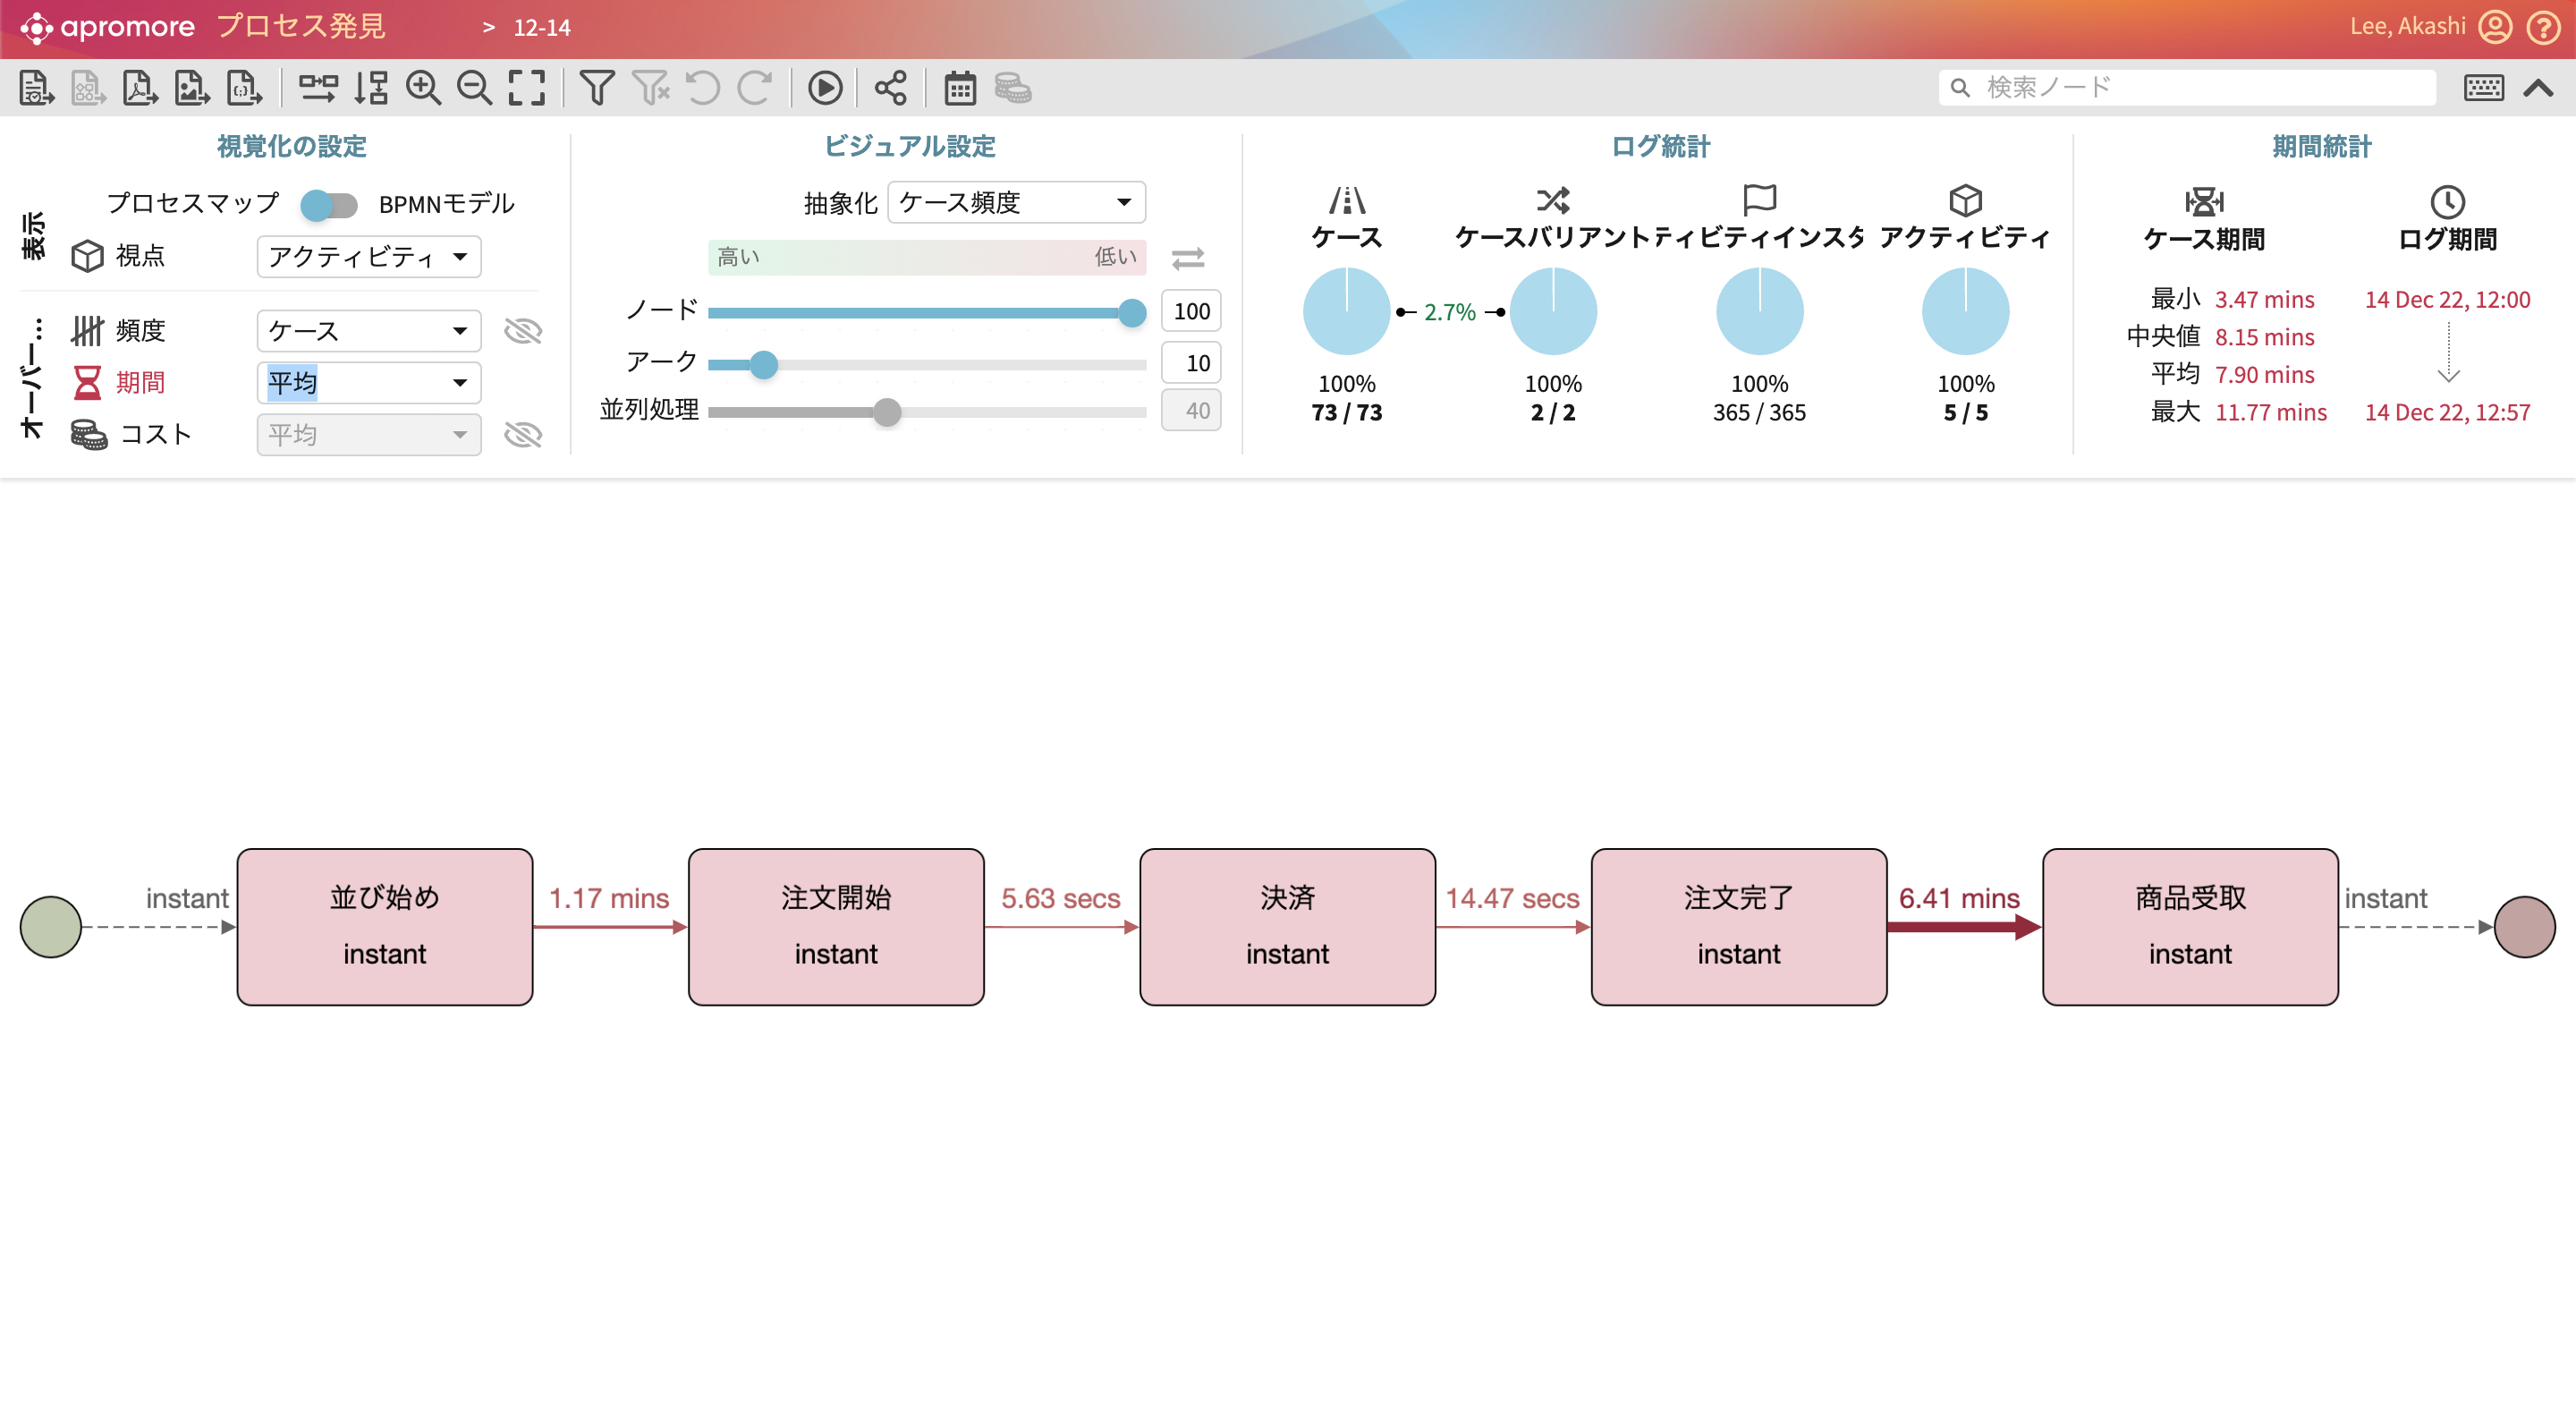
\includegraphics[width=15cm]{3.png}
  \caption{Apromoreの分析画面}
  \label{fig:3}
\end{figure}



\newpage

\subsection{関連研究}

店舗における行列を分析するために飲食店の形態を把握することやレジや受け取り口での
スタッフの人数の変更による影響などを参考にした。
こちらではスマートフォンなどでの事前注文決済を行うことで注文決済の待ち時間をゼロにすることは
非常に有効であるがそれと半面に店舗が混雑しキャパオーバーを起こす状況\cite{bibi2}が
あると指摘している。ここではモバイルオーダーを導入した店舗形態の評価を行うために様々な
パターンのモデルについて比較評価を行なっている。表\ref{table1}に店舗形態のパターンとその説明を示す。

\begin{table}[H]
 \begin{center}
   \caption{店舗形態のパターン}
  \begin{tabular}{|c|l|} \hline
1-1     & レジ1人、商品提供1人\\ \hline
2-1     & レジ2人、商品提供1人\\ \hline
2-1(IT) & レジ1人とITによるレジ、商品提供1人\\ \hline
  \end{tabular}
 \label{table1}
 \end{center}
\end{table}

ここではモバイルオーダーを1人のレジスタッフのような扱いをしており、モバイルオーダーで注文を
した利用客は来店するとレジへ行かずにそのまま受け取り口へ向かい商品の受け取り待ちをする。
またレジでスタッフが商品提供のところに利用客を流さずに
そのまま自分で商品を準備して処理をするということも想定している。
これによりサービス時間が短くなる傾向があることに触れており、論文では考察されていないが
作業を並行して行うことによるサービス時間の減少であると考えられる。
また、シミュレーションでは行列の人数が増えるほど混雑を嫌って並ばなくなる人が増えることや、
モバイルオーダーの導入によりレジでの混雑が減ったことにより、
混雑を避けていた利用客が利用することによる利用率の向上にも配慮が必要である。





\newpage

\section{研究内容}

\subsection{行列データの収集方法}
実店舗での行列計測については、近畿大学東大阪キャンパスにある近大をすすらんか(以下近大ラーメン)に承諾を得て行った。
近大ラーメンでは、レジの代わりに券売機を設置して食券を購入し半券を渡すと注文が通る仕組みとなっている。
近大ラーメンの利用者は、来店して列がない場合は待ち時間なしですぐに券売機にて食券を購入する。列があれば並び先頭になった際に券売機にて食券を購入し、
半券を渡し注文が終了すると待ちの行列に移動する。
ここでは具体的に列に並ぶわけではないが基本的に注文順に料理が受け渡される。
料理の準備ができると料理を受け取り、受け取り待ちの行列から抜ける。
行列計測から取得するタイムスタンプは、行列参加時間,注文開始時間,決済開始時間,注文完了時間,商品受け取り時間の5つである。さらに性別の区分やグループ人数別の区分のデータも取得する。
表\ref{table2}に近大ラーメンにおける店舗フローと取得するタイムスタンプの対応表を示す。

\begin{table}[H]
 \begin{center}
   \caption{近大ラーメンにおける店舗フローと取得するタイムスタンプの対応表}
   \begin{tabular}{|c|c|} \hline
店舗フロー      & タイムスタンプ \\ \hline \hline
列があれば並ぶ   & 行列参加時間 \\ \hline
券売機の先頭     & 注文開始時間 \\ \hline
券売機にお金投入  & 決済開始時間 \\ \hline
半券を渡す       & 注文完了時間 \\ \hline
料理を受け取る   & 商品受け取り時間 \\ \hline
  \end{tabular}
 \label{table2}
 \end{center}
\end{table}


行列の計測方法は、行列計測用のアプリケーション(以下ExpoGo)\cite{bibi3}を用いて行う。
ExpoGoのUIを図\ref{fig:4}に示す。
図\ref{fig:4}の左の画面は行列計測のホーム画面であり、
ピンク色の丸で囲まれた「行列」を押下すると真ん中の行列参加計測画面に遷移し、
緑色の丸で囲まれた「注文決済」を押下すると右の注文決済計測画面に遷移する。
複数台のデバイスからでもリアルタイムに計測が可能となっており、
行列の計測は3人以上が望ましいが、2人でも問題なく計測可能となっている。
2人の役割分担は、1人は行列参加者を計測し何人で来たのかをメモする。
もう1人は、注文開始時間、決済開始時間、注文完了時間、商品受け取り時間を計測する。


\begin{figure}[H]
  \centering
  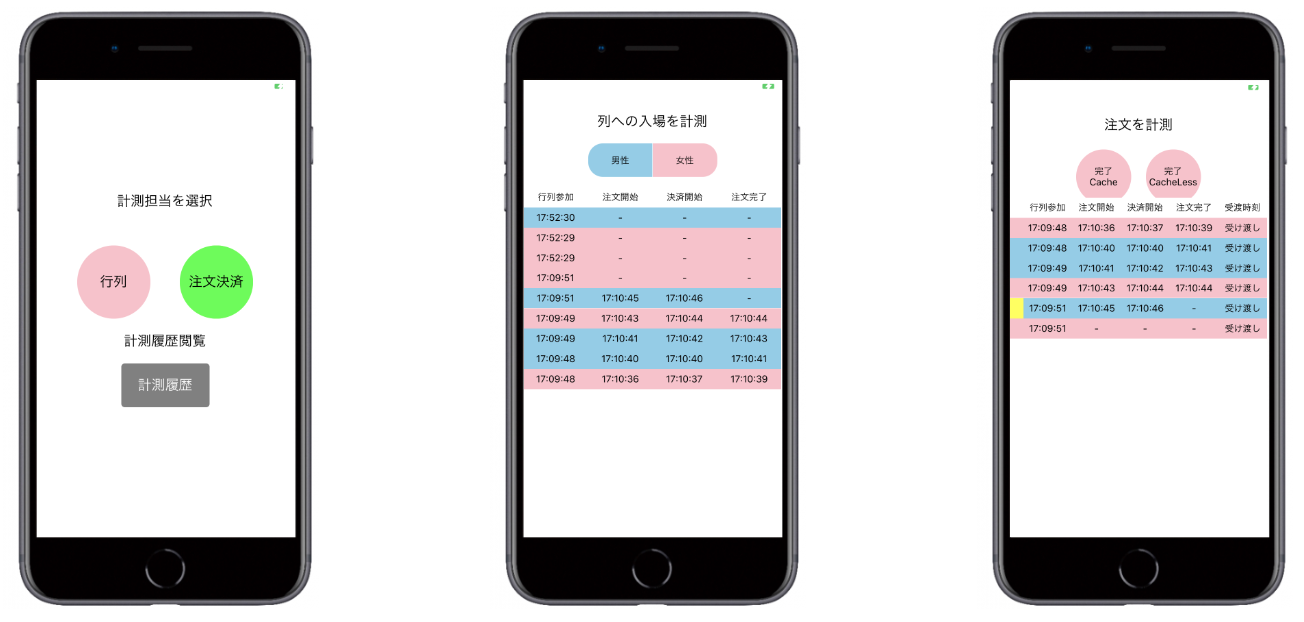
\includegraphics[width=14.5cm]{4.png}
  \caption{ExpoG0(左からホーム画面、行列参加、注文決済)}
\scriptsize(出典:事前注文・事前決済プラットフォームの開発と導入による待ち行列の評価-事前注文・事前決済プラットフォームの開発.藤井遼.)
  \label{fig:4}
\end{figure}



取得するタイムスタンプのデータとデータキーの一覧を表\ref{table3}に示す。
また、集合Tの各差分を求める事で行列時間、注文時間、決済時間、商品受取待ち時間を算出できるので
表\ref{table4}に差分関係を示す。



\begin{table}[H]
 \begin{center}
   \caption{取得するタイムスタンプのデータとデータキーの一覧}
   \begin{tabular}{|c|l|l|l|} \hline
ti & データキー     & 取得データ      & データ例 \\ \hline \hline
t1 & queueing\_at  & 行列参加時間    & 2022-07-21 10:00:00 \\ \hline
t2 & ordered\_at   & 注文開始時間    & 2022-07-21 10:01:00 \\ \hline
t3 & paymented\_at & 決済開始時間    & 2022-07-21 10:02:00 \\ \hline
t4 & serviced\_at  & 注文完了時間    & 2022-07-21 10:03:00 \\ \hline
t5 & handed\_at    & 商品受け取り時間 & 2022-07-21 10:05:00 \\ \hline
  \end{tabular}
 \label{table3}
 \end{center}
\end{table}



\begin{table}[H]
 \begin{center}
   \caption{算出する項目と差分関係}
   \begin{tabular}{|c|c|} \hline
算出する項目 & 差分関係 \\ \hline \hline
行列時間 & $t2-t1$ \\ \hline
注文時間 & $t3-t2$ \\ \hline
決済時間 & $t4-t3$ \\ \hline
商品受取待ち時間 & $t5-t4$ \\ \hline
  \end{tabular}
 \label{table4}
 \end{center}
\end{table}





\newpage
\subsection{行列データの分析計画}
図\ref{fig:5}のように近大ラーメンにて行列を計測しイベントログを得る。
取得したイベントログのデータをCSVファルに変換し、
Apromoreにアップロードしてプロセスマイニングを行う。
プロセスマイニングでプロセスを可視化するために最低限必要となるイベントログのデータ項目は、
一連の作業をひも付ける「ケースID」、各活動を示す「アクティビティ」、
活動が実行された日時の「タイムスタンプ」の3つである。そのほかにも自由に追加することができる。
今回の計測では、行列参加時間、注文開始時間、決済開始時間、注文完了時間、商品受け取り時間の5つの区分に加えて性別の区分やグループ人数別の区分のデータも取得するので、
性別とグループ人数の項目を追加してデータを取得しCSVファイルを作成した。
CSVファイルに変換したデータをプロセスマイニングを用いて分析するとプロセスマップが
自動的に生成され行列時間、注文時間、決済時間、商品受取待ち時間などの平均時間等が表示され、
さらにケースIDやイベント属性、ケース属性、時間軸などの条件を指定してフィルタリングを行うことで、注文する際の性別間での差や、グループ人数間での違いによって生じる差を分析する。

\begin{figure}[H]
  \centering
  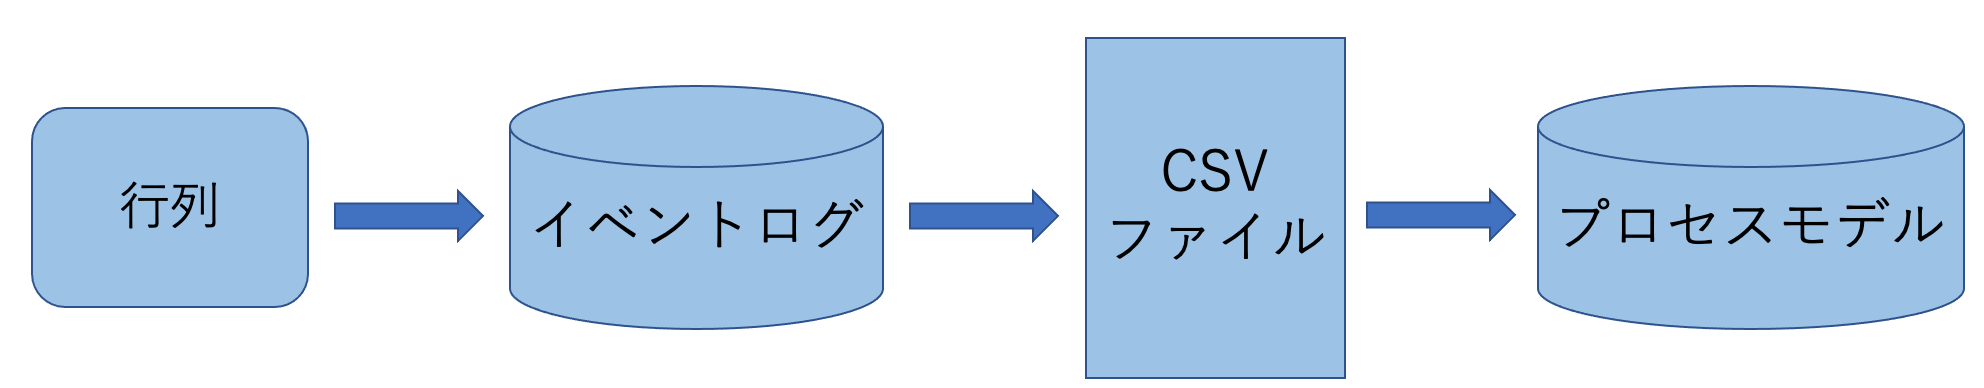
\includegraphics[width=14.5cm]{5.png}
  \caption{プロセスマイニングを行うまでの全体像}
  \label{fig:5}
\end{figure}






\newpage

\section{結果・考察}

\subsection{プロセスマイニングを用いた行列データの分析}

%------------------------------------------------------------------
近大ラーメンで計測した日時と計測した項目の一覧を表\ref{table5}に示す。
7月の行列計測は行列参加時間、注文開始時間、決済開始時間、注文完了時間、商品受け取り時間の
5つの区分に分けて計測した。
12月の行列計測は7月に計測した上記の5つの区分に加えて、
新たに性別とグループ人数の項目も追加して計測を行った。

\begin{table}[H]
 \begin{center}
   \caption{計測日程と計測項目}
   \begin{tabular}{|c|c|c|c|c|c|c|c|} \hline
日時 & 行列参加 & 注文開始 & 決済開始 & 注文完了 & 商品受取 & グループ人数 & 性別 \\ \hline \hline
2022/07/08 12:00〜13:00 & ○ & ◯ & ◯ & ◯ & ◯ & × & × \\ \hline
2022/07/11 12:00〜13:00 & ○ & ◯ & ◯ & ◯ & ◯ & × & × \\ \hline
2022/07/12 12:00〜13:00 & ○ & ◯ & ◯ & ◯ & ◯ & × & × \\ \hline
2022/12/14 12:00〜13:00 & ○ & ◯ & ◯ & ◯ & ◯ & ◯ & ◯ \\ \hline
2022/12/16 12:00〜13:00 & ○ & ◯ & ◯ & ◯ & ◯ & ◯ & ◯ \\ \hline
  \end{tabular}
 \label{table5}
 \end{center}
\end{table}
%------------------------------------------------------------------




\subsubsection{行列データの分析}
%------------------------------------------------------------------
7月,12月に計測したデータのプロセスマップを
図\ref{fig:708},図\ref{fig:711},図\ref{fig:712},図\ref{fig:1214},図\ref{fig:1216}に示す。左から順に行列に並んだ時間、注文にかかった時間、決済から注文完了にかかった時間、
商品の受取待ち時間の各平均時間を表している。

\begin{figure}[H]
  \centering
  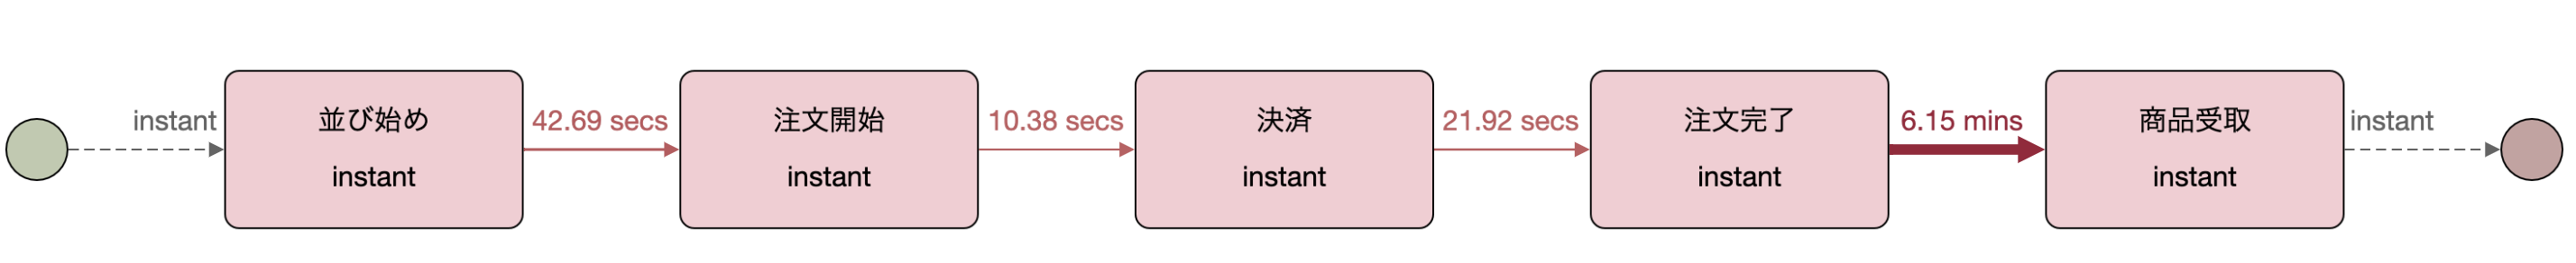
\includegraphics[width=15cm]{708.png}
  \caption{計測日時:7/8 12:00〜13:00,来店数:52人の各計測項目の平均時間}
  \label{fig:708}
\end{figure}

\begin{figure}[H]
  \centering
  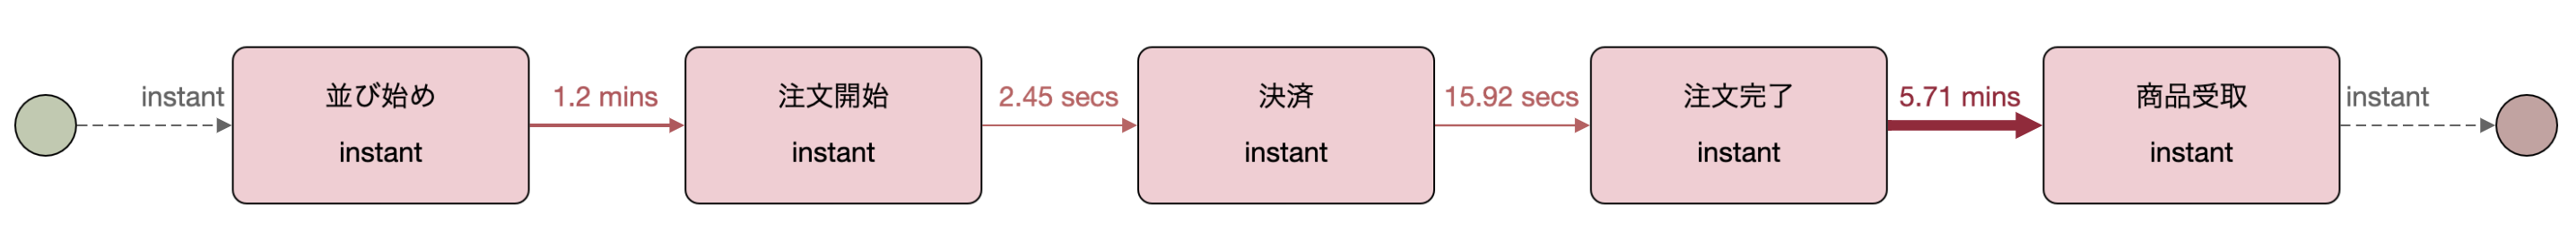
\includegraphics[width=15cm]{711.png}
  \caption{計測日時:7/11 12:00〜13:00,来店数:49人の各計測項目の平均時間}
  \label{fig:711}
\end{figure}

\begin{figure}[H]
  \centering
  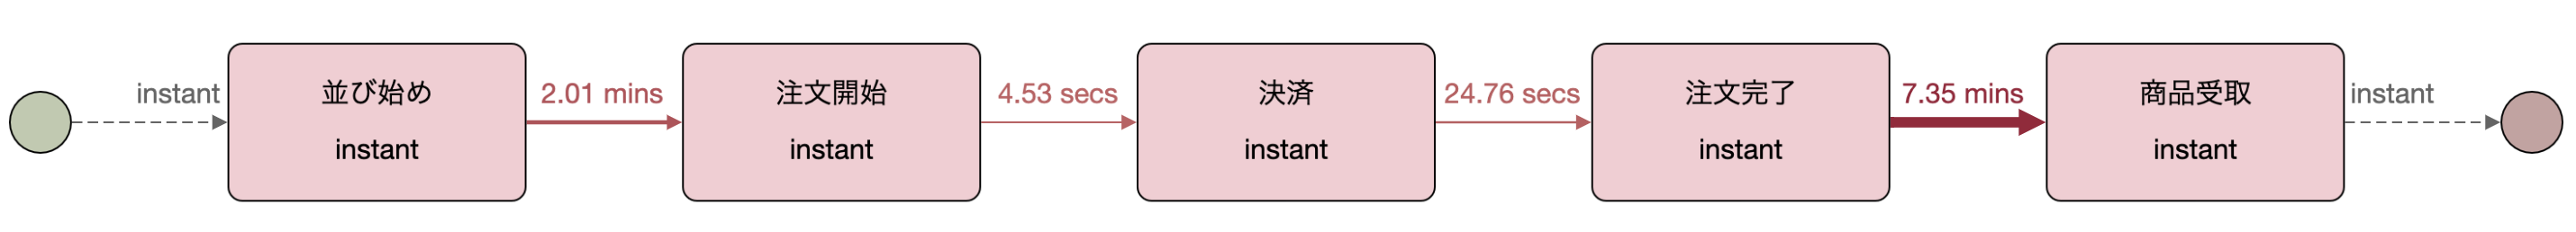
\includegraphics[width=15cm]{712.png}
  \caption{計測日時:7/12 12:00〜13:00,来店数:75人の各計測項目の平均時間}
  \label{fig:712}
\end{figure}

\begin{figure}[H]
  \centering
  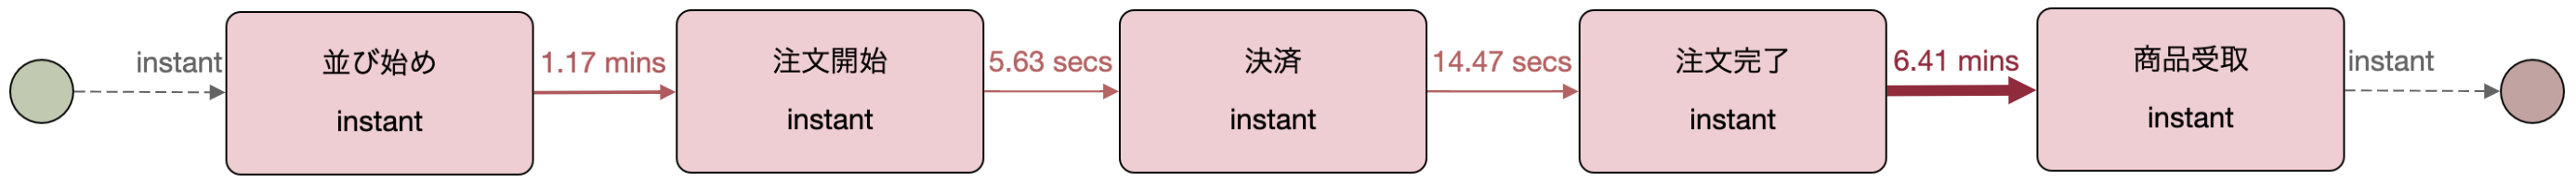
\includegraphics[width=15cm]{1214.png}
  \caption{計測日時:12/14 12:00〜13:00,来店数:73人の各計測項目の平均時間}
  \label{fig:1214}
\end{figure}

\begin{figure}[H]
  \centering
  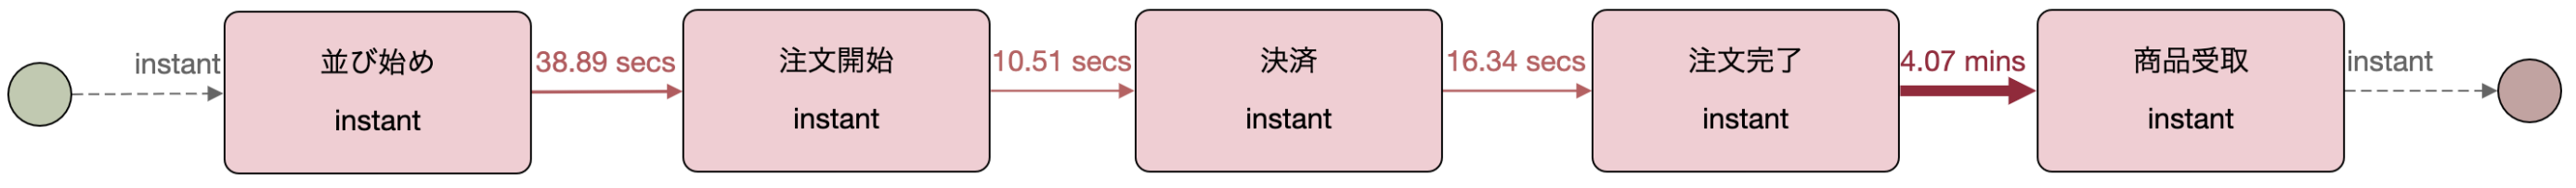
\includegraphics[width=15cm]{1216.png}
  \caption{計測日時:12/16 12:00〜13:00,来店数:61人の各計測項目の平均時間}
  \label{fig:1216}
\end{figure}
%------------------------------------------------------------------




\subsubsection{フィルタリングしたデータ分析}
%------------------------------------------------------------------
5日間を通して混雑したと思われる12:15〜12:30の時間軸の図と各計測項目の平均時間を示す。
\begin{itemize}
\item 7/8 12:15〜12:30のデータを図\ref{fig:708a},図\ref{fig:708b}
\item 7/11 12:15〜12:30のデータを図\ref{fig:711a},図\ref{fig:711b}
\item 7/12 12:15〜12:30のデータを図\ref{fig:712a},図\ref{fig:712b}
\item 12/14 12:15〜12:30のデータを図\ref{fig:1214a},図\ref{fig:1214b}
\item 12/16 12:15〜12:30のデータを図\ref{fig:1216a},図\ref{fig:1216b}
\end{itemize}

図\ref{fig:708a},図\ref{fig:711a},図\ref{fig:712a},図\ref{fig:1214a},
図\ref{fig:1216a}は12:15〜12:30以外のイベントログデータをフィルタリングしているのを表している。
図\ref{fig:708b},図\ref{fig:711b},図\ref{fig:712b},図\ref{fig:1214b},
図\ref{fig:1216b}は12:15〜12:30のデータのプロセスマップであり、
左から順に行列に並んだ時間、注文にかかった時間、決済から注文完了にかかった時間、
商品の受取待ち時間の各平均時間を表している。

\begin{figure}[H]
  \centering
  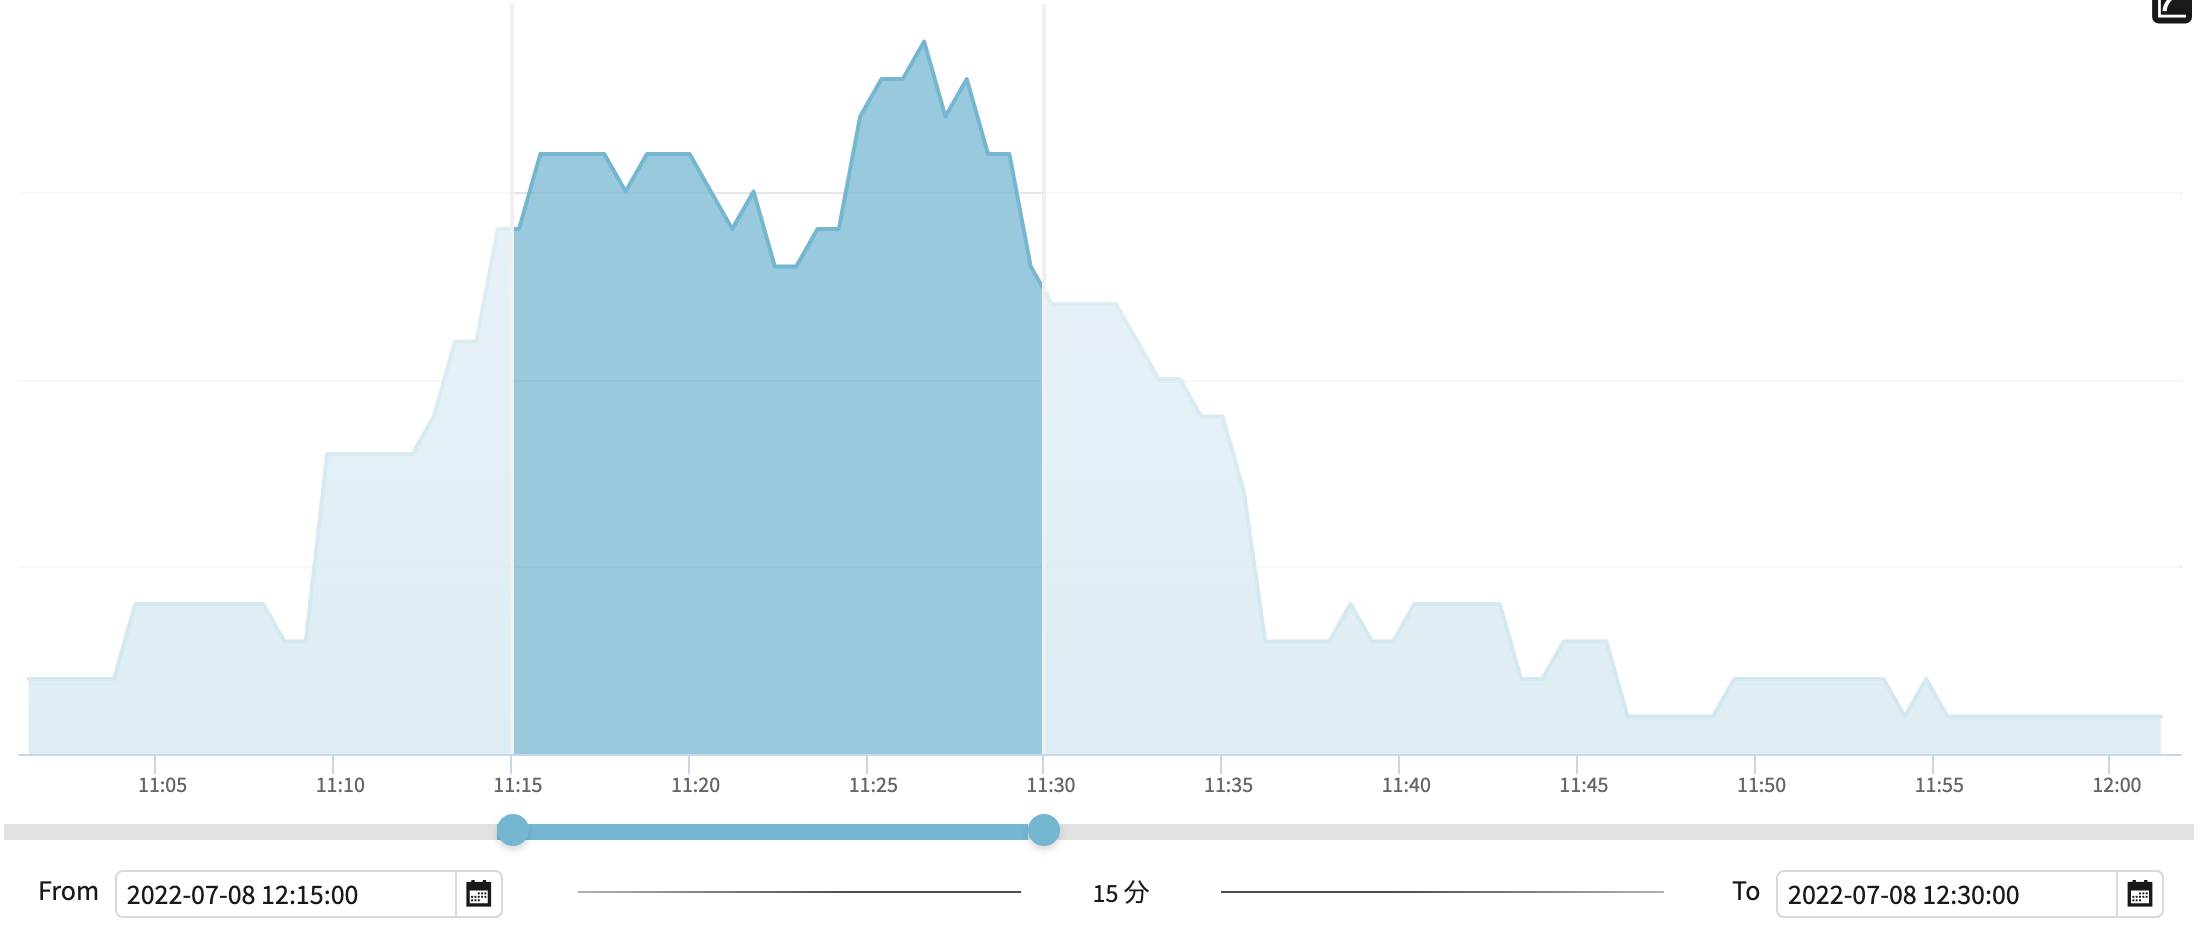
\includegraphics[width=14cm]{708a.png}
  \caption{計測日時:7/8 12:15〜12:30,来店数:37人の時間軸}
  \label{fig:708a}
\end{figure}

\begin{figure}[H]
  \centering
  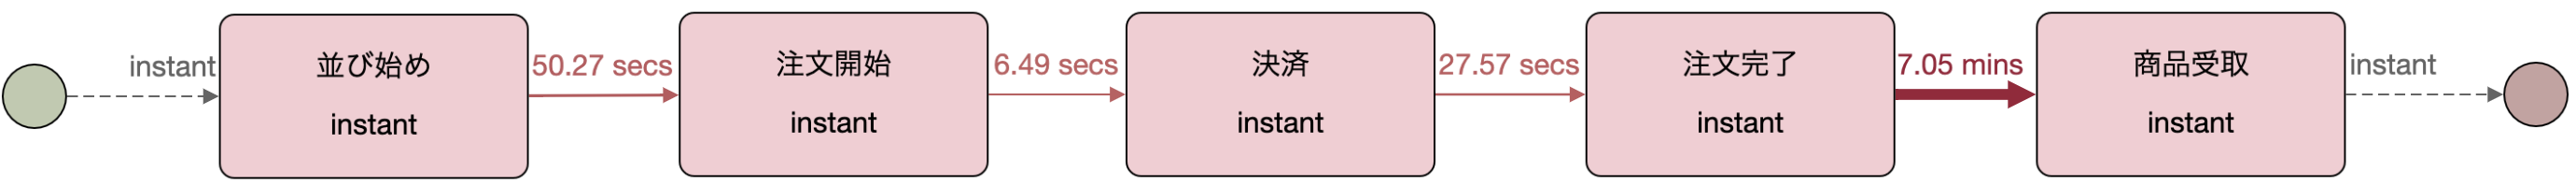
\includegraphics[width=15cm]{708b.png}
  \caption{計測日時:7/8 12:15〜12:30,来店数:37人の各計測項目の平均時間}
  \label{fig:708b}
\end{figure}


\begin{figure}[H]
  \centering
  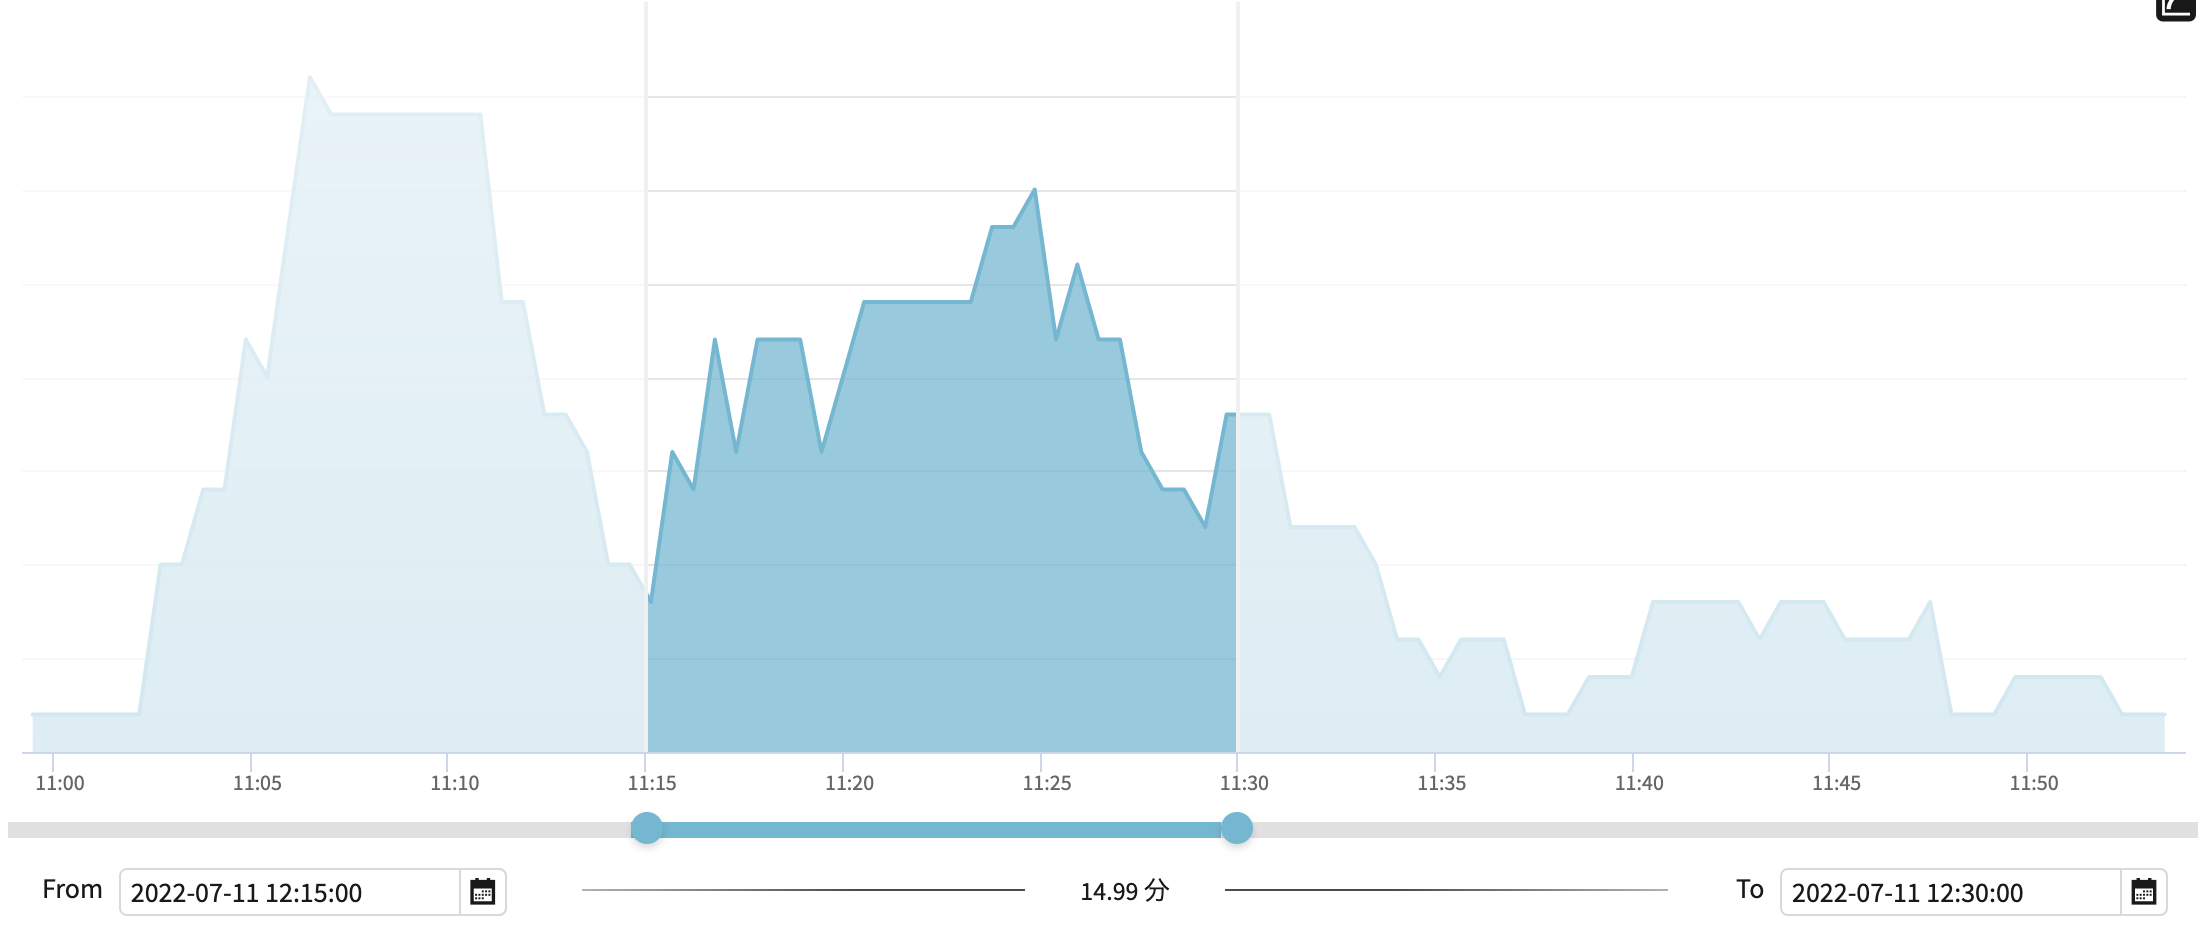
\includegraphics[width=14cm]{711a.png}
  \caption{計測日時:7/11 12:15〜12:30,来店数:27人の時間軸}
  \label{fig:711a}
\end{figure}

\begin{figure}[H]
  \centering
  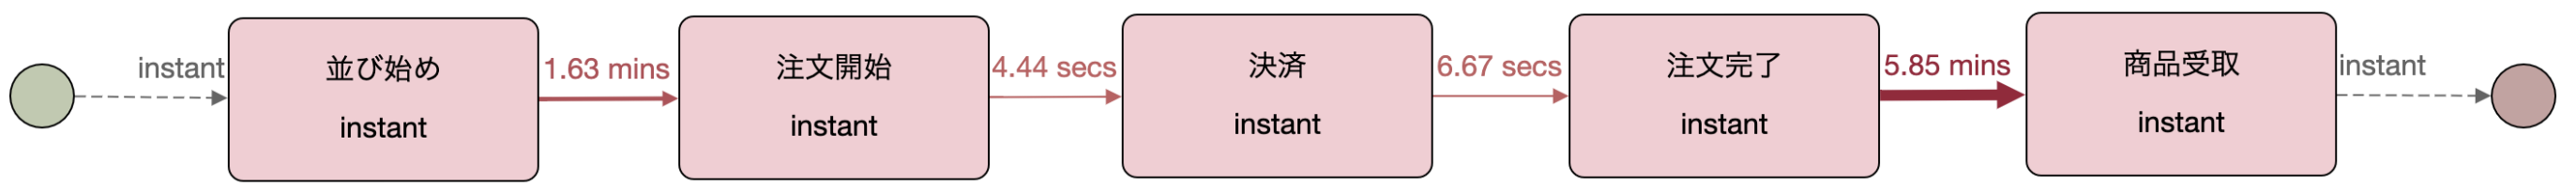
\includegraphics[width=15cm]{711b.png}
  \caption{計測日時:7/11 12:15〜12:30,来店数:27人の各計測項目の平均時間}
  \label{fig:711b}
\end{figure}


\begin{figure}[H]
  \centering
  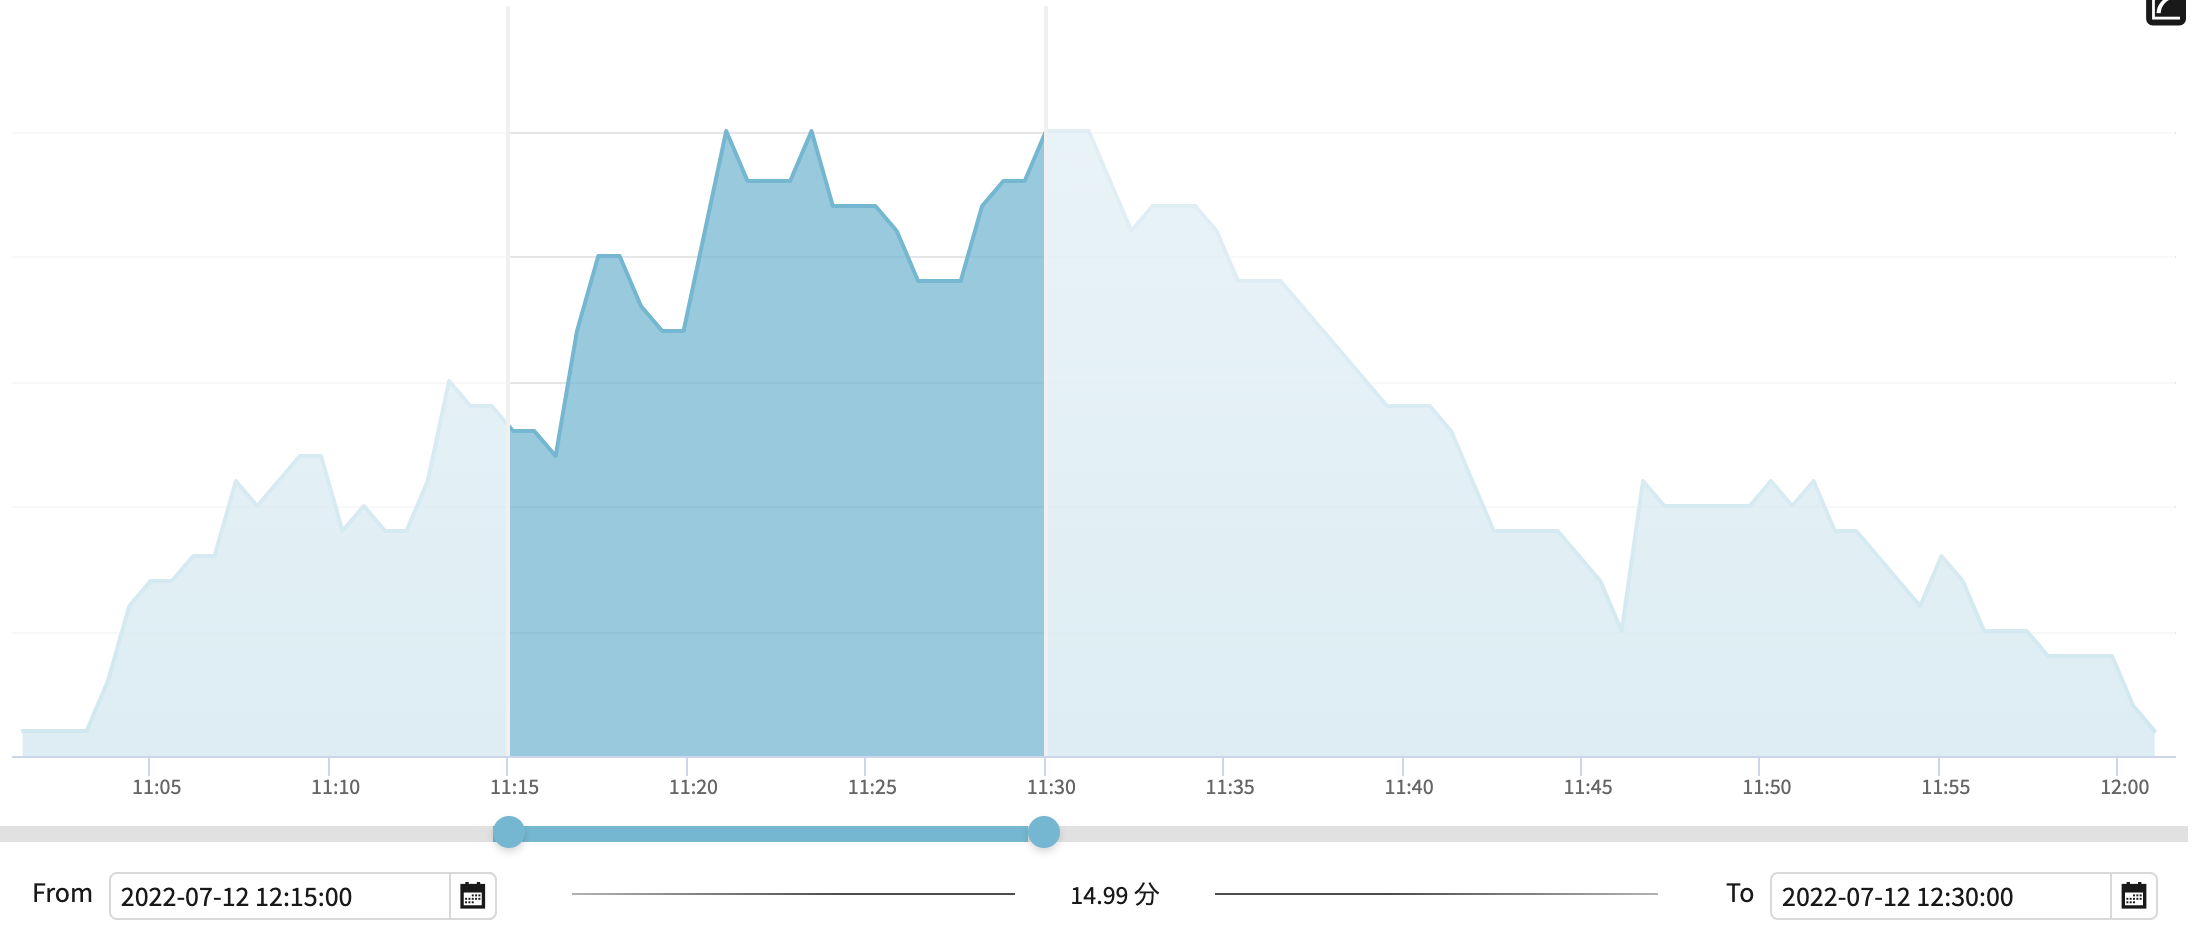
\includegraphics[width=14cm]{712a.png}
  \caption{計測日時:7/12 12:15〜12:30,来店数:43人の時間軸}
  \label{fig:712a}
\end{figure}

\begin{figure}[H]
  \centering
  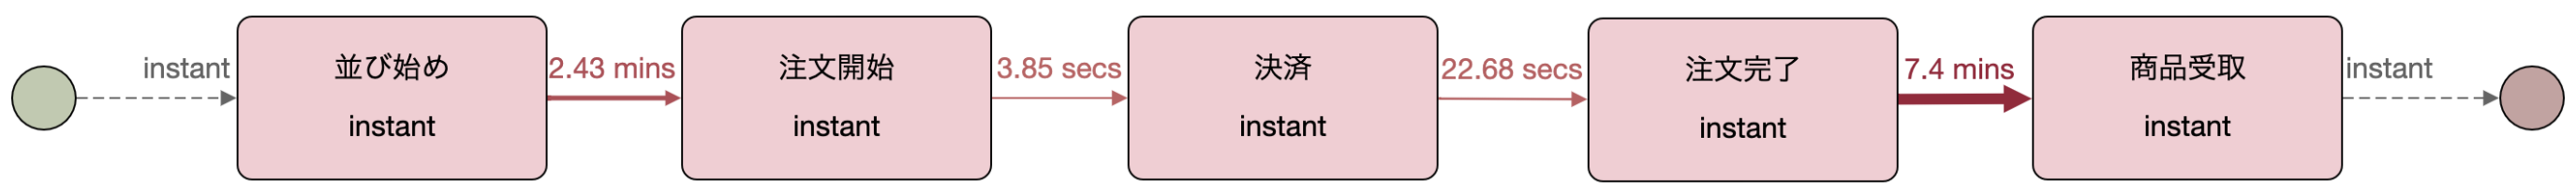
\includegraphics[width=15cm]{712b.png}
  \caption{計測日時:7/12 12:15〜12:30,来店数:43人の各計測項目の平均時間}
  \label{fig:712b}
\end{figure}


\begin{figure}[H]
  \centering
  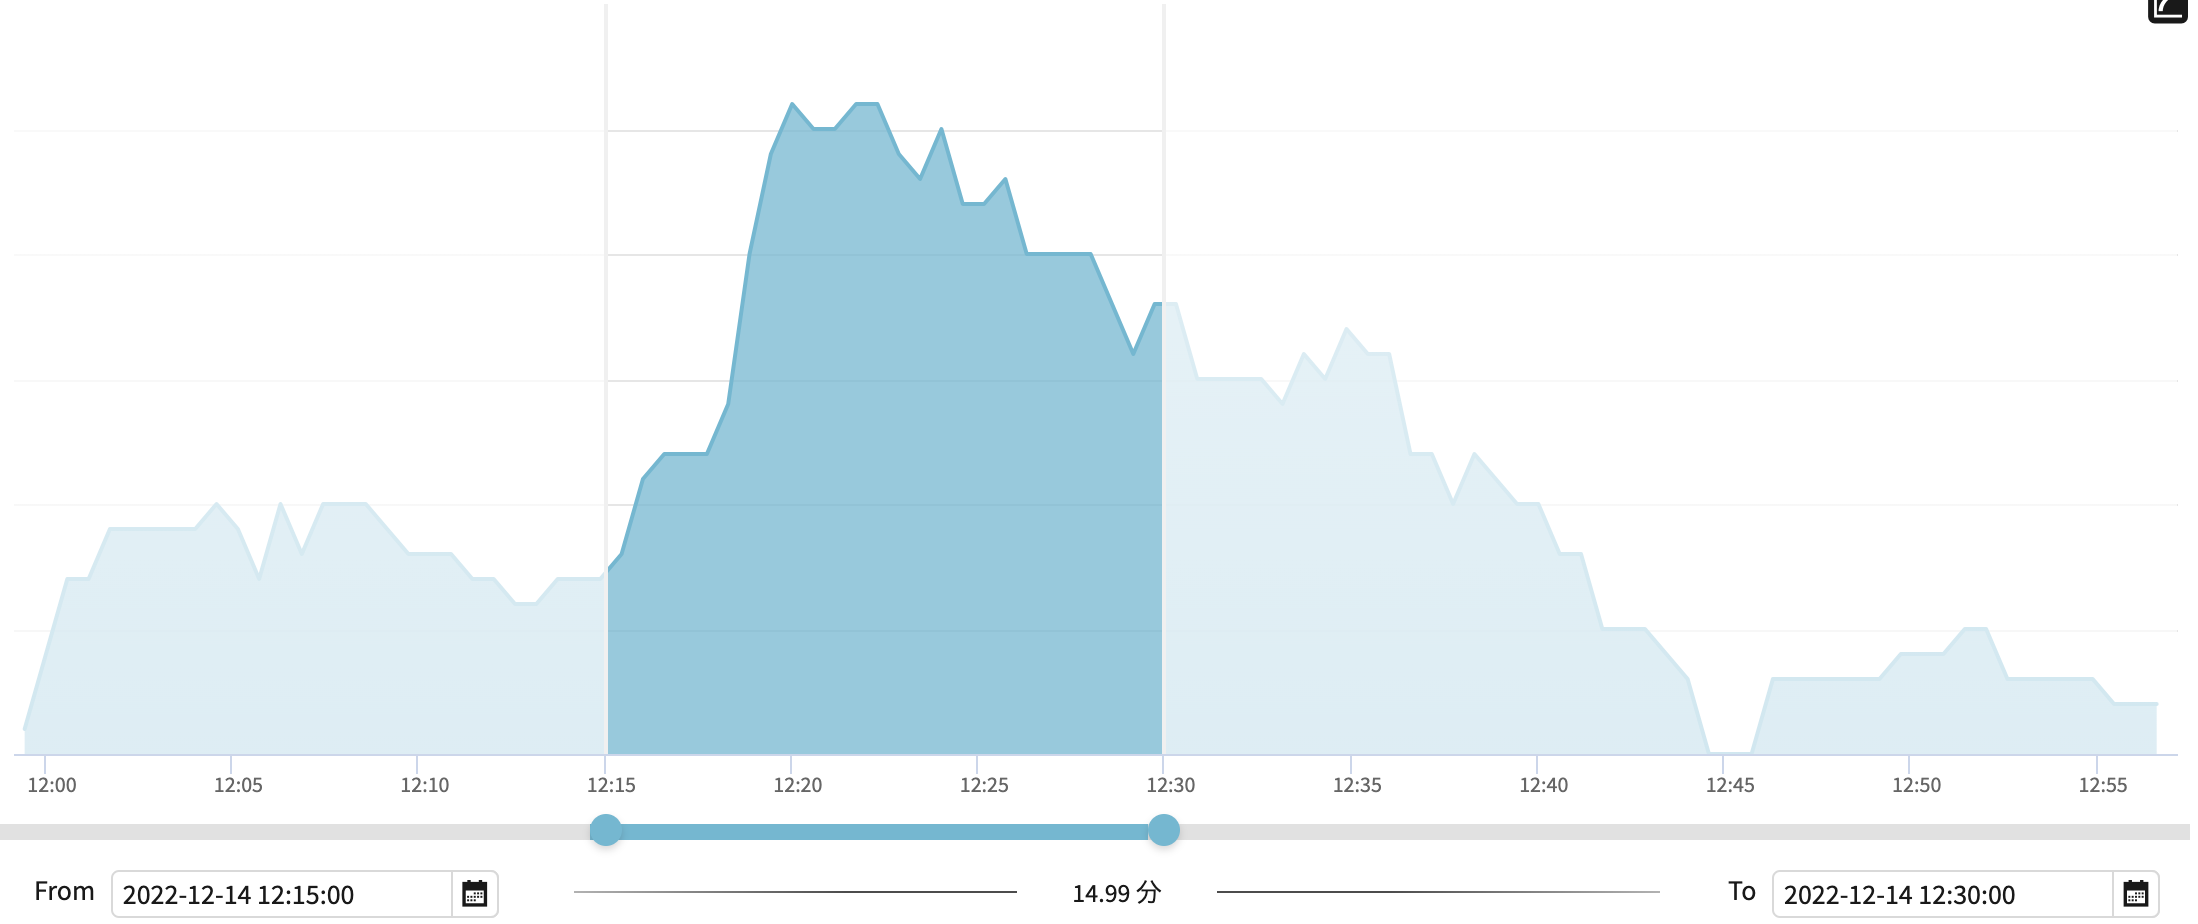
\includegraphics[width=15cm]{1214a.png}
  \caption{計測日時:12/14 12:15〜12:30,来店数:38人の時間軸}
  \label{fig:1214a}
\end{figure}
\begin{figure}[H]
  \centering
  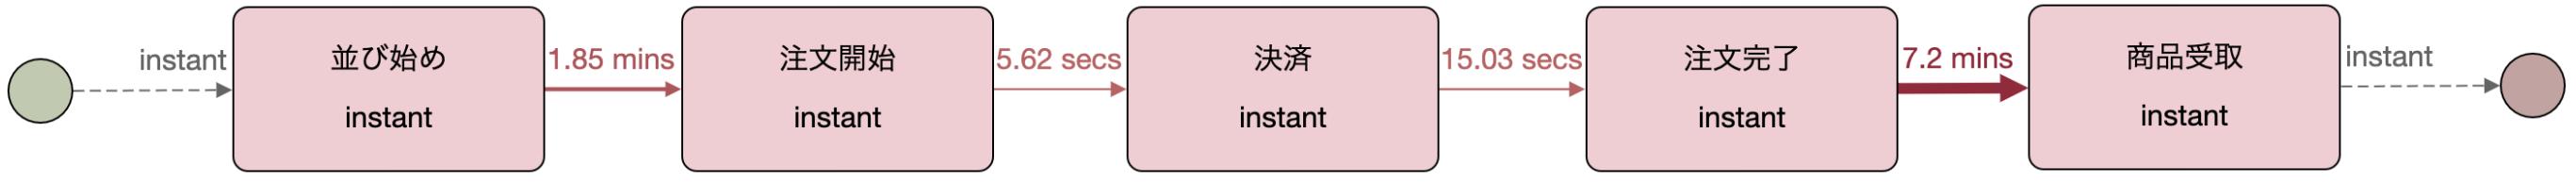
\includegraphics[width=15cm]{1214b.png}
  \caption{計測日時:12/14 12:15〜12:30,来店数:38人の各計測項目の平均時間}
  \label{fig:1214b}
\end{figure}


\begin{figure}[H]
  \centering
  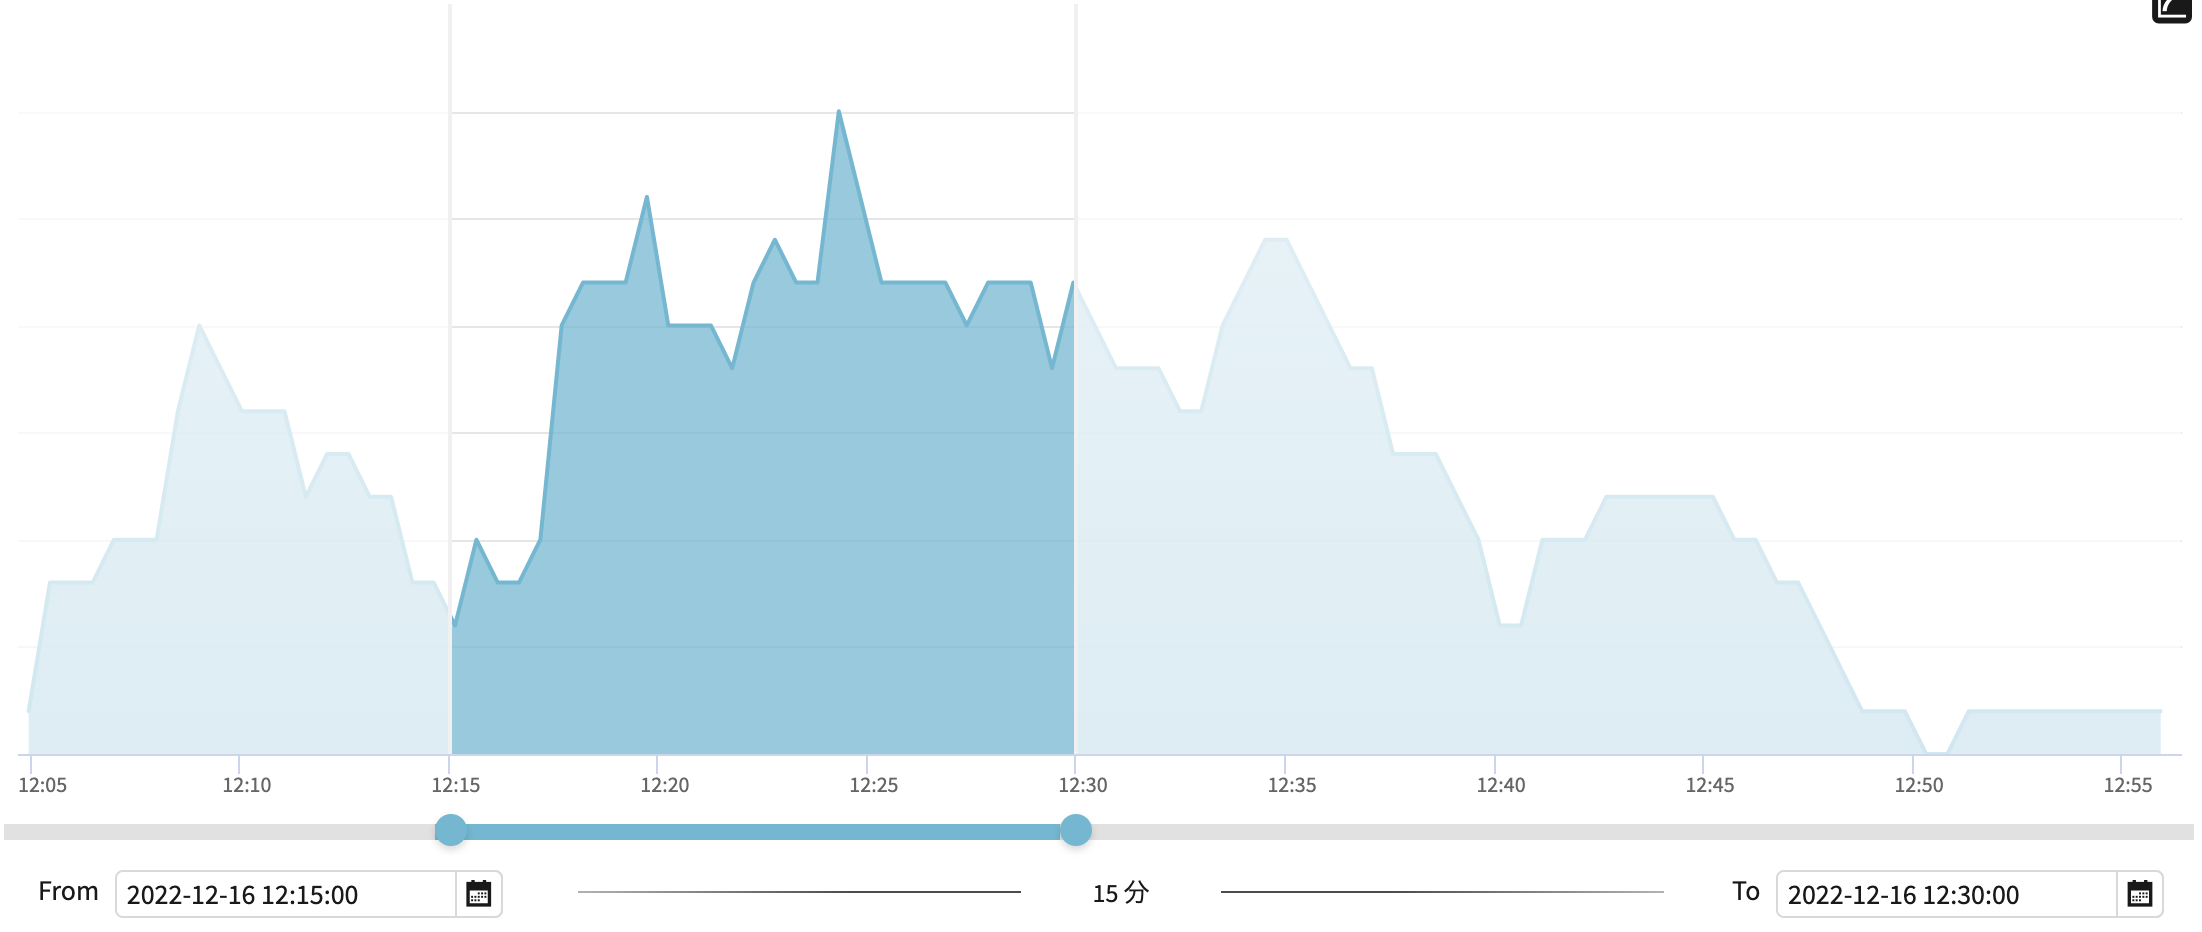
\includegraphics[width=15cm]{1216a.png}
  \caption{計測日時:12/16 12:15〜12:30,来店数:28人の時間軸}
  \label{fig:1216a}
\end{figure}
\begin{figure}[H]
  \centering
  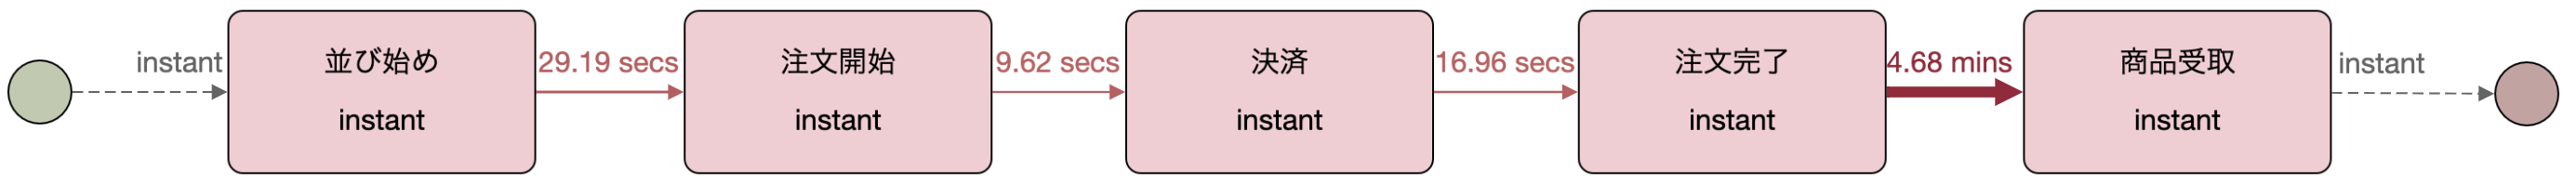
\includegraphics[width=15cm]{1216b.png}
  \caption{計測日時:12/16 12:15〜12:30,来店数:28人の各計測項目の平均時間}
  \label{fig:1216b}
\end{figure}

%------------------------------------------------------------------




\newpage
%------------------------------------------------------------------
5日間の12:00〜13:00と12:15〜12:30における来店数やその割合、
各計測項目の平均時間を表\ref{table6}に示す。

\begin{table}[H]
 \begin{center}
   \caption{時間軸でフィルタリングした各計測項目の平均時間}
   \begin{tabular}{|c|c|c|c|c|c|c|} \hline
日時 & 来店数 & 割合 & 行列時間 & 注文時間 & 決済時間 & 商品受取待ち時間 \\ \hline \hline
2022/07/08 12:00〜13:00 & 52 & 100\% & 43秒    & 10秒 & 22秒 & 6分9秒 \\ \hline
2022/07/08 12:15〜12:30 & 37 & 71\%  & 50秒    & 6秒 & 28秒  & 7分3秒 \\ \hline \hline

2022/07/11 12:00〜13:00 & 49 & 100\% & 1分12秒 & 3秒 & 16秒 & 5分43秒 \\ \hline
2022/07/11 12:15〜12:30 & 27 & 55\%  & 1分38秒 & 4秒 & 7秒   & 5分51秒 \\ \hline \hline

2022/07/12 12:00〜13:00 & 75 & 100\% & 2分1秒  & 5秒  & 25秒 & 7分21秒 \\ \hline
2022/07/12 12:15〜12:30 & 47 & 63\%  & 2分26秒 & 4秒 & 27秒  & 7分24秒 \\ \hline \hline

2022/12/14 12:00〜13:00 & 73 & 100\% & 1分10秒 & 6秒 & 14秒 & 6分25秒 \\ \hline
2022/12/14 12:15〜12:30 & 38 & 52\%  & 1分38秒 & 6秒 & 15秒  & 7分32秒 \\ \hline \hline

2022/12/16 12:00〜13:00 & 61 & 100\% & 39秒 & 11秒  & 16秒 & 4分4秒 \\ \hline
2022/12/16 12:15〜12:30 & 28 & 46\%  & 28秒 & 10秒 & 17秒   & 4分34秒 \\ \hline
  \end{tabular}
 \label{table6}
 \end{center}
\end{table}


表\ref{table6}より、5日間いずれも12:15〜12:30までの15分の間に、1時間の間に来店する客の半数前後が来店している事から12:15〜12:30までの15分の間は混雑している時間だと伺う事ができる。
行列時間は5日中4日が12:15〜12:30の方が長くなり、
来店数が増加するに連れ行列時間も長くなる傾向にある事が分かる。
注文時間や決済時間は券売機と客の1-1の関係なので来店数によらないものだと考えられる。
商品受取待ち時間も5日中5日が12:15〜12:30の方が長くなり、
行列時間と同様に来店数が増加するに連れ商品受取待ち時間も長くなる傾向にある事が分かる。
%------------------------------------------------------------------




\subsubsection{区分別のデータ分析}

%------------------------------------------------------------------
7月に計測した際より性別の区分、グループ人数ごとの区分を追加し二日間計測した。
12/14 12:00〜13:00の行列計測データの性別フィルターログ選択画面を図\ref{fig:1214mw}に示す。
真ん中より少し上に位置する水色の部分のチェック部分で性別を切り替えて
フィルターログを得ることができる。
男女それぞれの各計測項目の平均時間を図\ref{fig:man1},図\ref{fig:woman1}に示す。
図\ref{fig:man1},図\ref{fig:woman1}は12:00〜13:00の性別のデータのプロセスマップであり、左から順に行列に並んだ時間、注文にかかった時間、決済から注文完了にかかった時間、
商品の受取待ち時間の各平均時間を表している。

\begin{figure}[H]
  \centering
  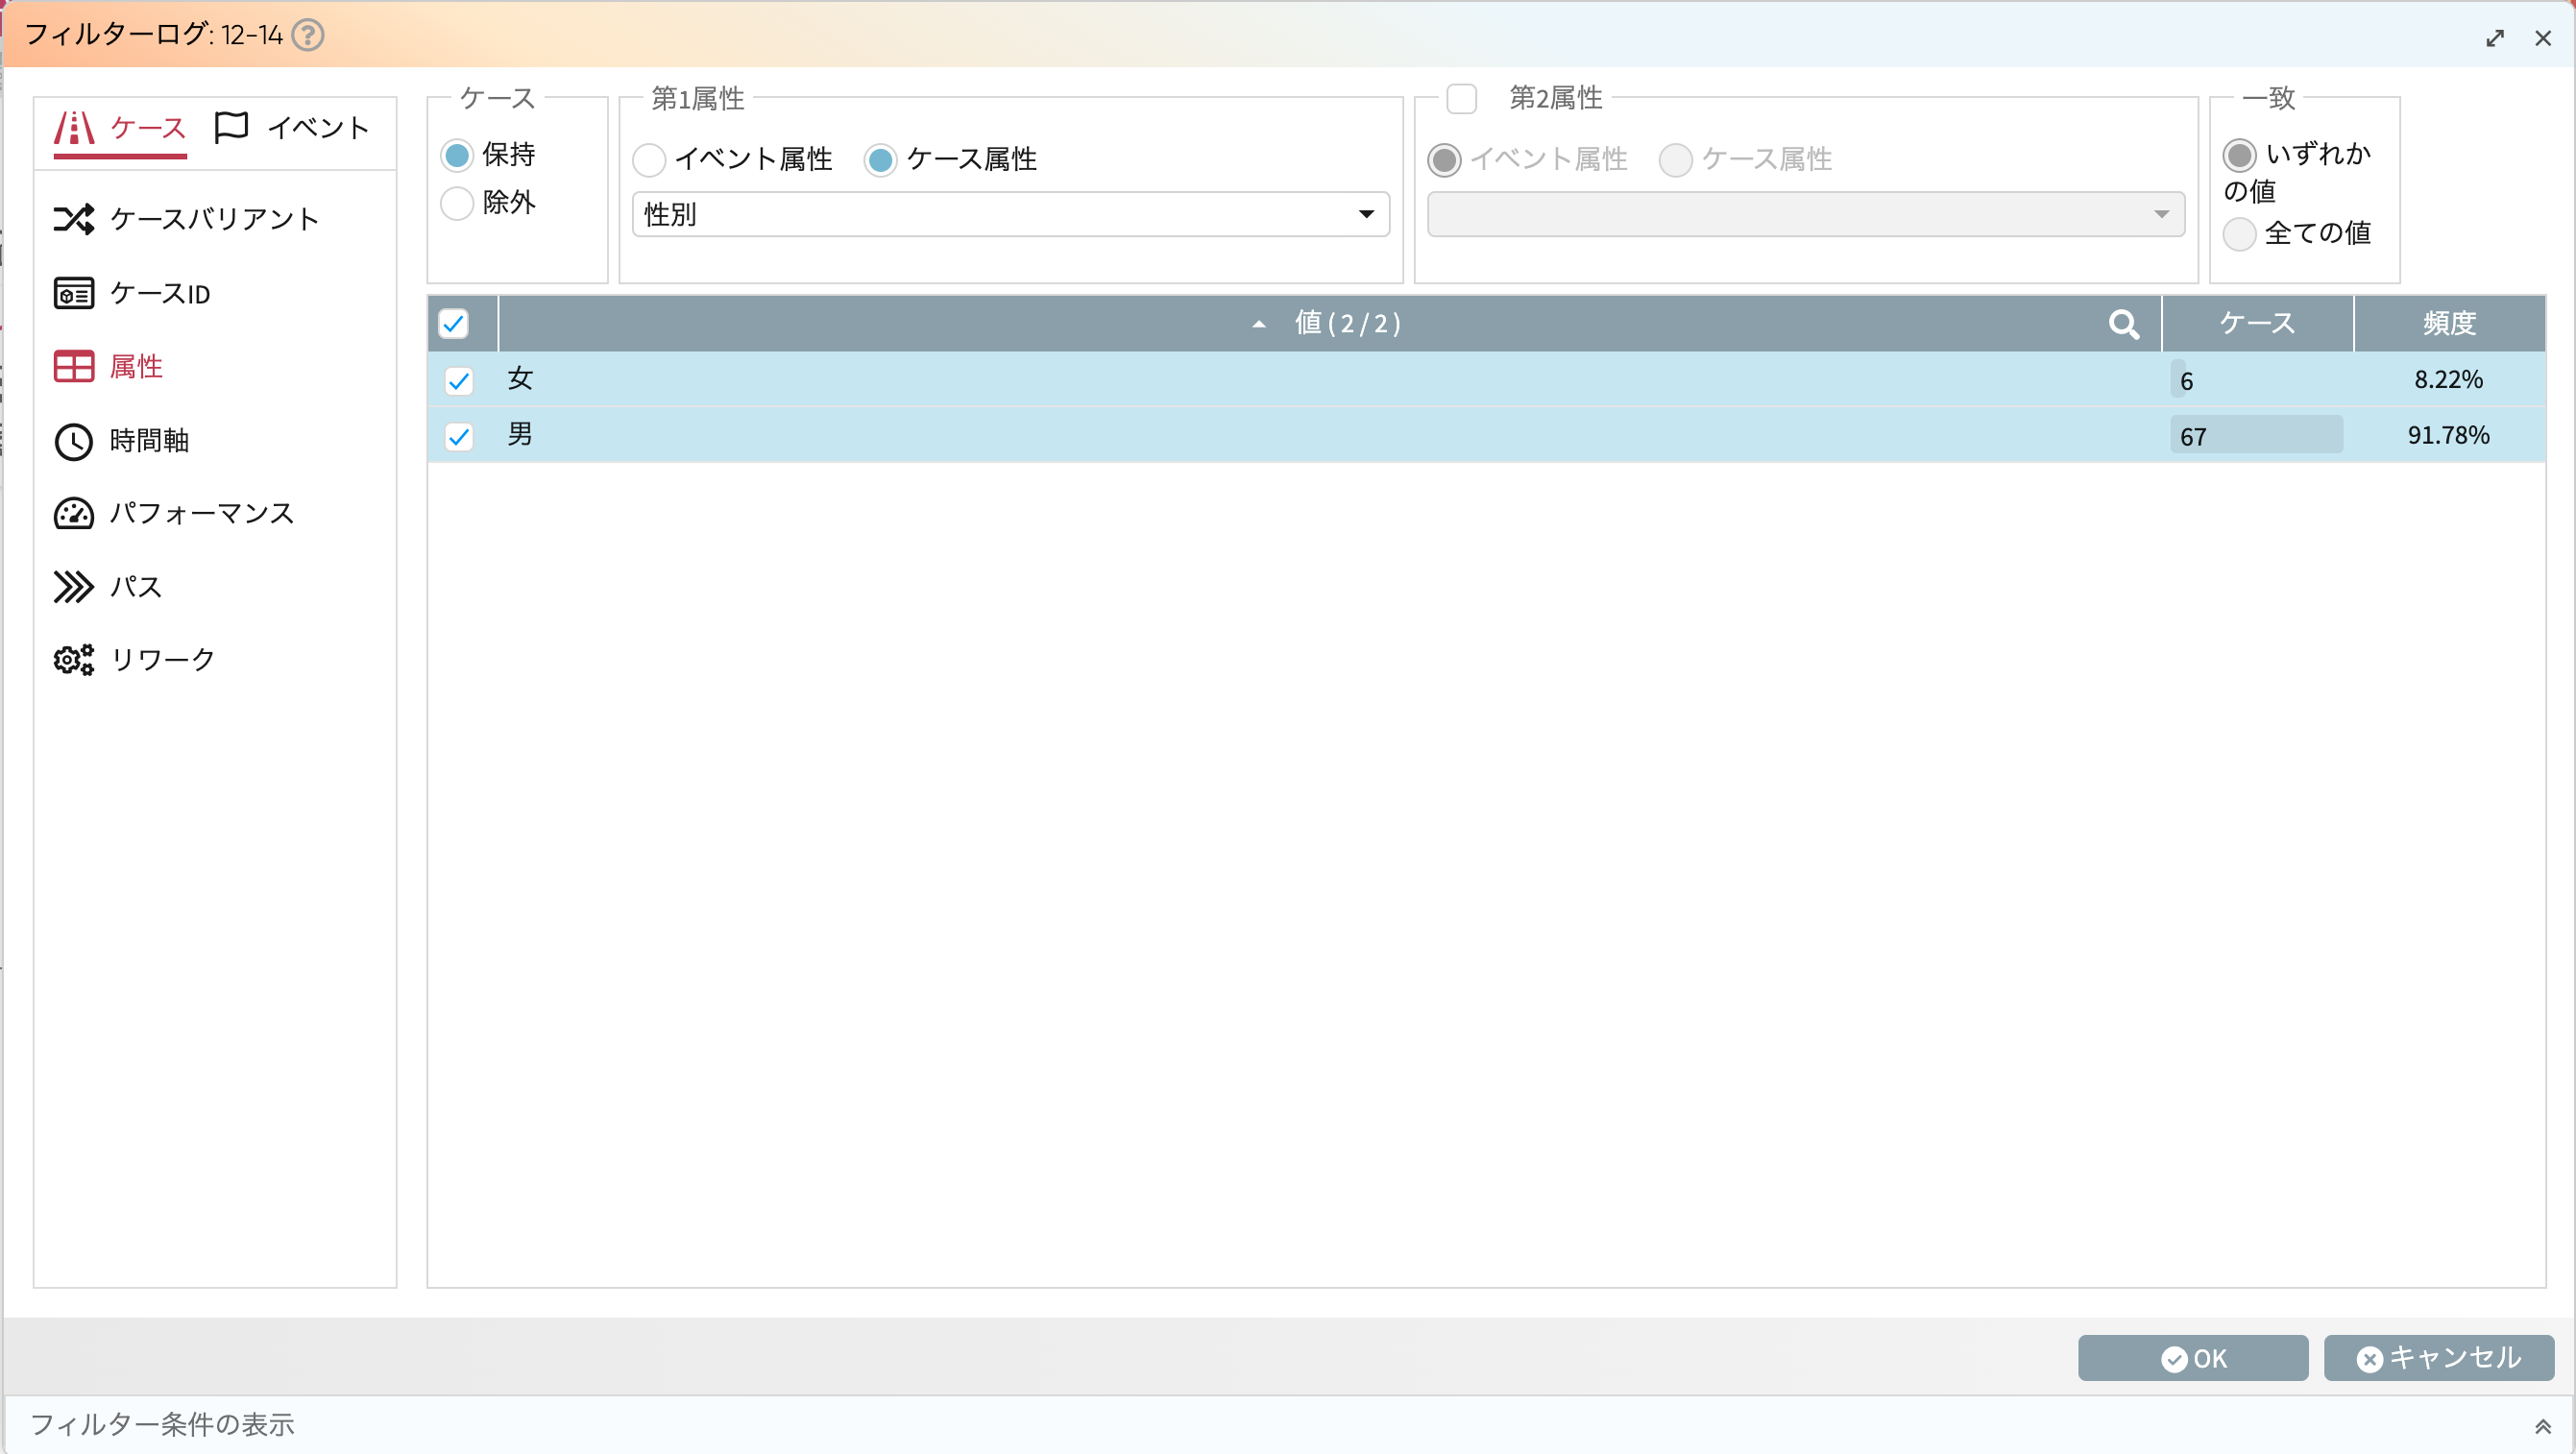
\includegraphics[width=15cm]{1214mw.png}
  \caption{計測日時:12/14 12:00〜13:00,ケース属性の性別フィルターログ選択画面}
  \label{fig:1214mw}
\end{figure}

\begin{figure}[H]
  \centering
  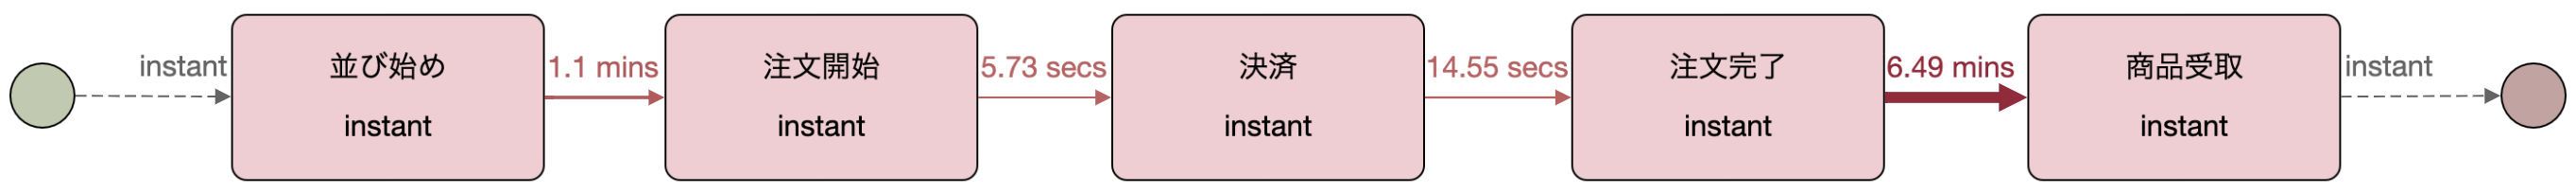
\includegraphics[width=15cm]{man1.png}
  \caption{計測日時:12/14 12:00〜13:00,性別:男,来店数:67人の各計測項目の平均時間}
  \label{fig:man1}
\end{figure}
  
\begin{figure}[H]
  \centering
  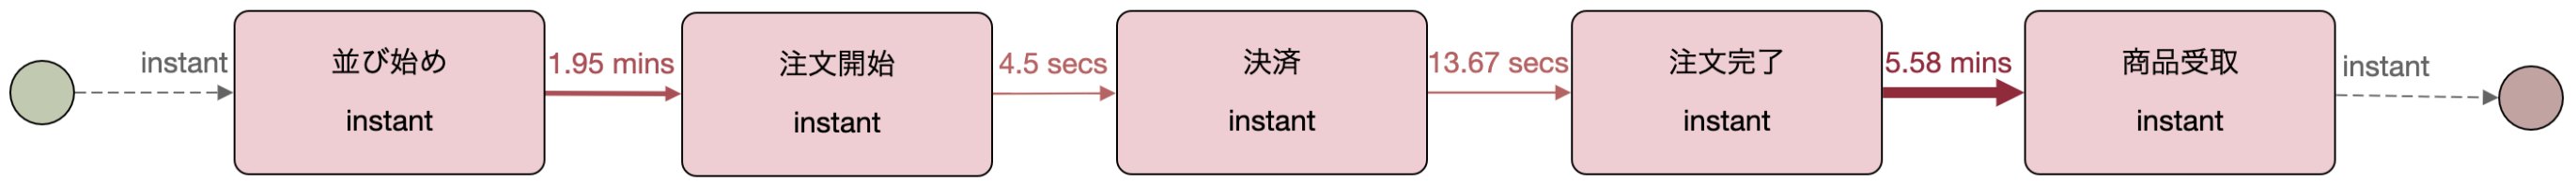
\includegraphics[width=15cm]{woman1.png}
  \caption{計測日時:12/14 12:00〜13:00,性別:女,来店数:6人の各計測項目の平均時間}
  \label{fig:woman1}
\end{figure}


12/14 12:00〜13:00の行列計測データのグループ人数フィルターログ選択画面を図\ref{fig:1214123}に示す。
真ん中より少し上に位置する水色の部分のチェック部分でグループ人数を切り替えて
フィルターログを得ることができる。
グループ人数それぞれの各計測項目の平均時間を
図\ref{fig:1-3a},図\ref{fig:2-3a},図\ref{fig:3-3a}に示す。
図\ref{fig:1-3a},図\ref{fig:2-3a},図\ref{fig:3-3a}は12:00〜13:00の
グループ人数別のデータのプロセスマップであり、左から順に行列に並んだ時間、
注文にかかった時間、決済から注文完了にかかった時間、
商品の受取待ち時間の各平均時間を表している。

\begin{figure}[H]
  \centering
  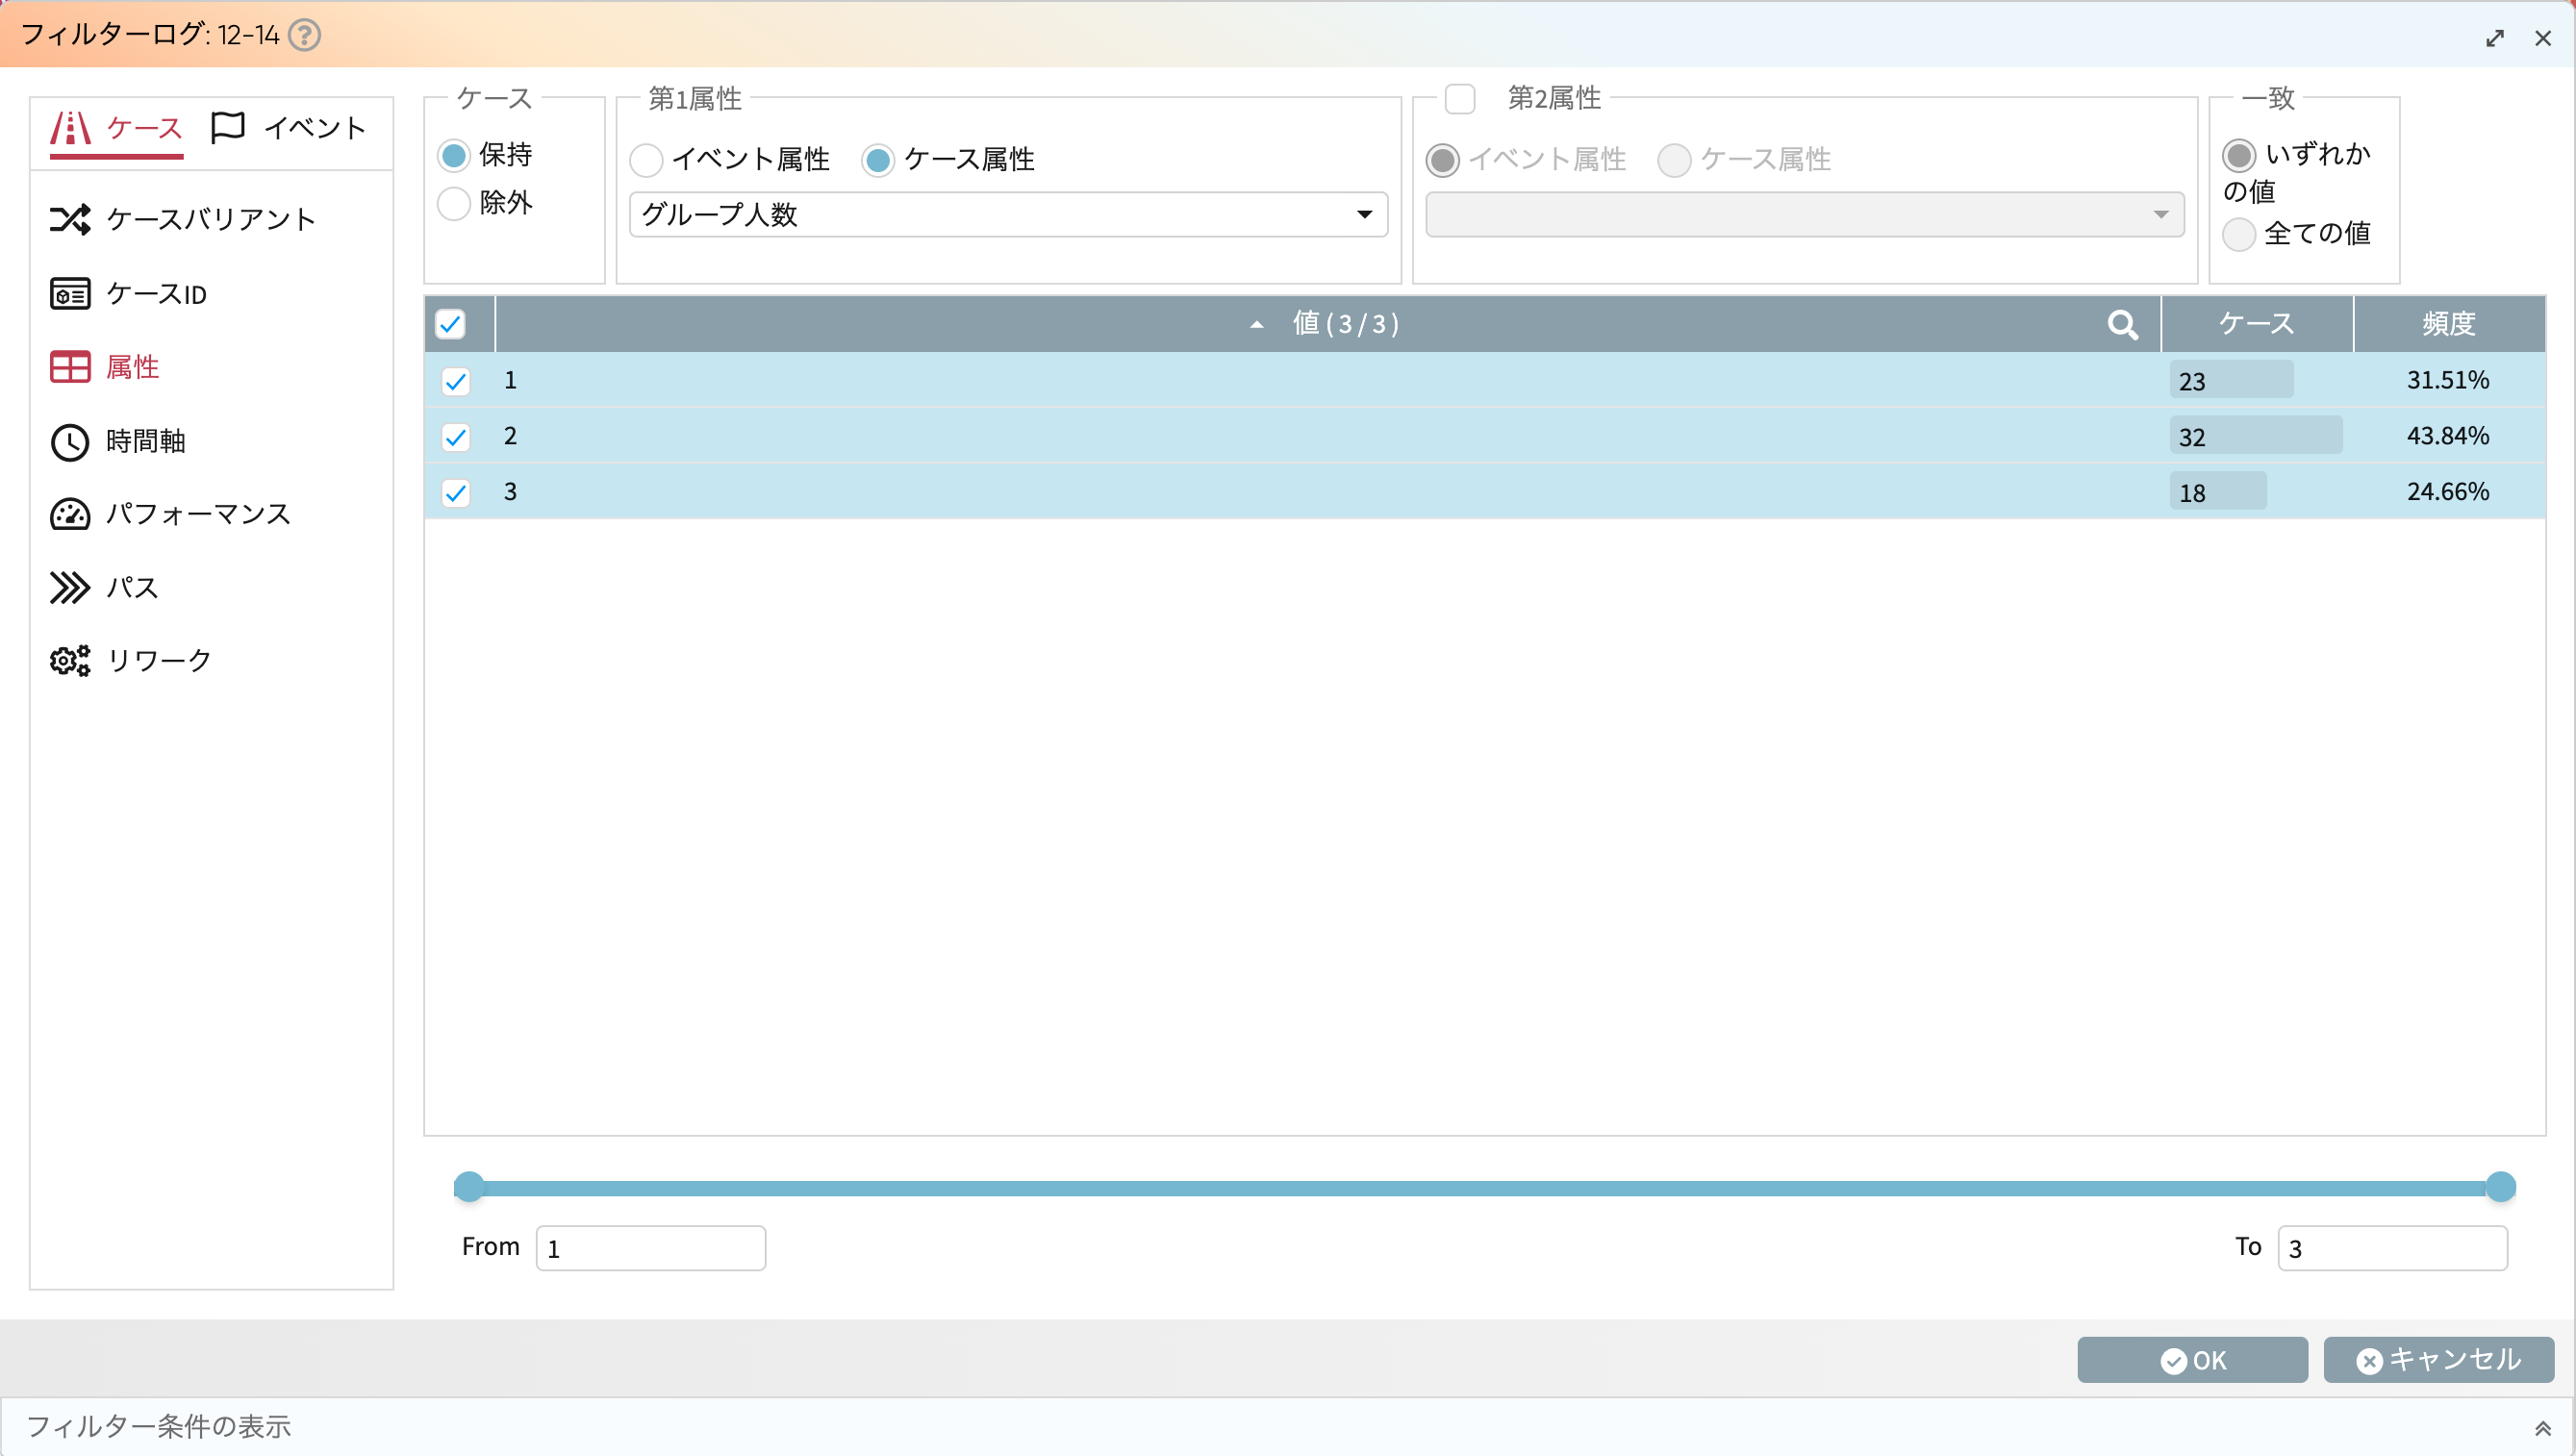
\includegraphics[width=15cm]{1214123.png}
  \caption{計測日時:12/14 12:00〜13:00,ケース属性のグループ人数フィルターログ選択画面}
  \label{fig:1214123}
\end{figure}

\begin{figure}[H]
  \centering
  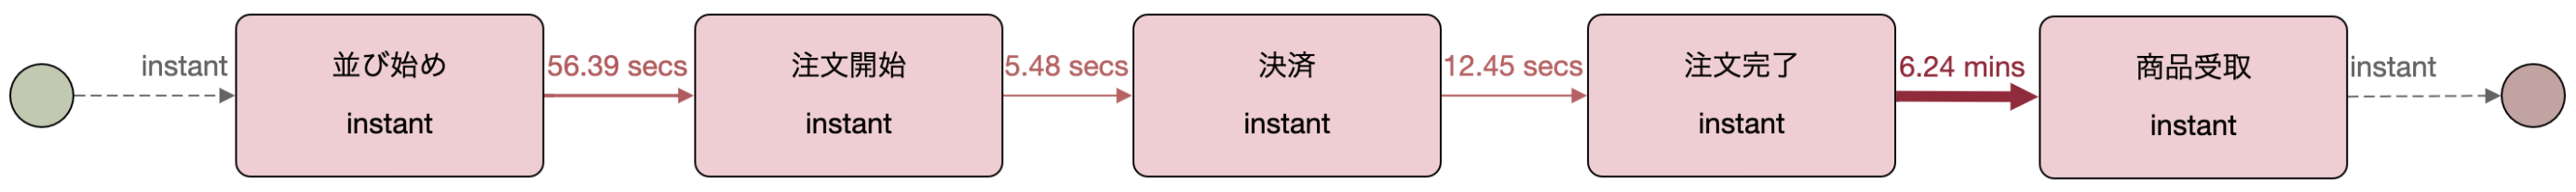
\includegraphics[width=15cm]{1-3a.png}
  \caption{計測日時:12/14 12:00〜13:00,グループ人数:1,来店数:23人の各計測項目の平均時間}
  \label{fig:1-3a}
\end{figure}

\begin{figure}[H]
  \centering
  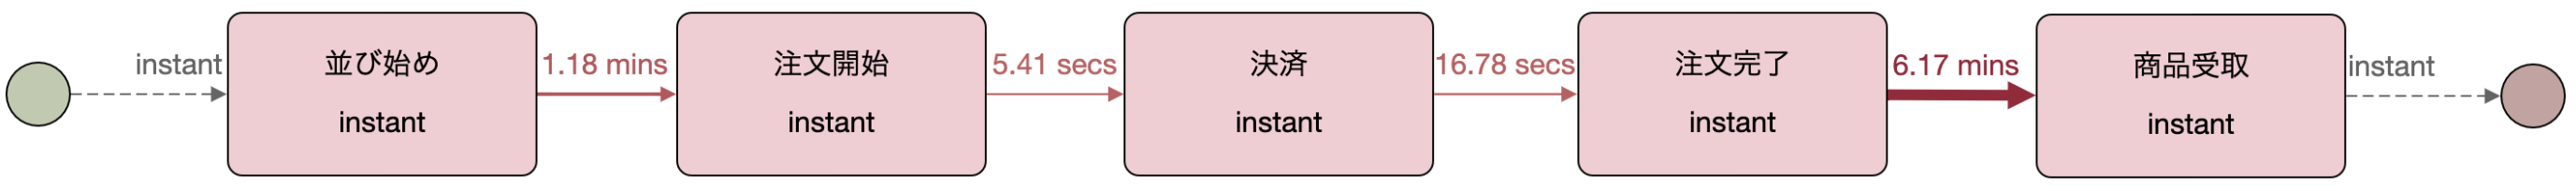
\includegraphics[width=15cm]{2-3a.png}
  \caption{計測日時:12/14 12:00〜13:00,グループ人数:2,来店数:32人の各計測項目の平均時間}
  \label{fig:2-3a}
\end{figure}

\begin{figure}[H]
  \centering
  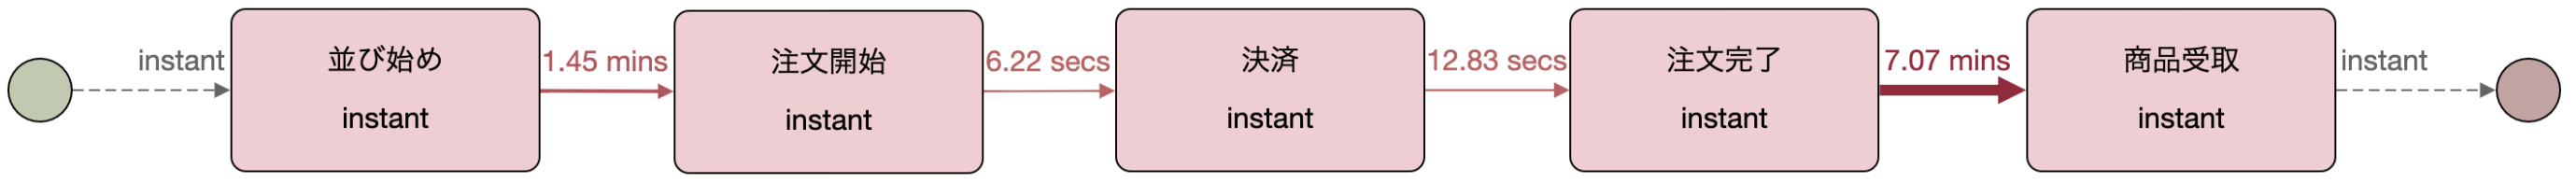
\includegraphics[width=15cm]{3-3a.png}
  \caption{計測日時:12/14 12:00〜13:00,グループ人数:3,来店数:18人の各計測項目の平均時間}
  \label{fig:3-3a}
\end{figure}
%------------------------------------------------------------------





%------------------------------------------------------------------
12/16 12:00〜13:00の行列計測データの性別フィルターログ選択画面を図\ref{fig:1216mw}に示す。
真ん中より少し上に位置する水色の部分のチェック部分で性別を切り替えて
フィルターログを得ることができる。
男女それぞれの各計測項目の平均時間を図\ref{fig:man2},図\ref{fig:woman2}に示す。
図\ref{fig:man2},図\ref{fig:woman2}は12:00〜13:00の男女のデータのプロセスマップであり、左から順に行列に並んだ時間、注文にかかった時間、決済から注文完了にかかった時間、
商品の受取待ち時間の各平均時間を表している。

\begin{figure}[H]
  \centering
  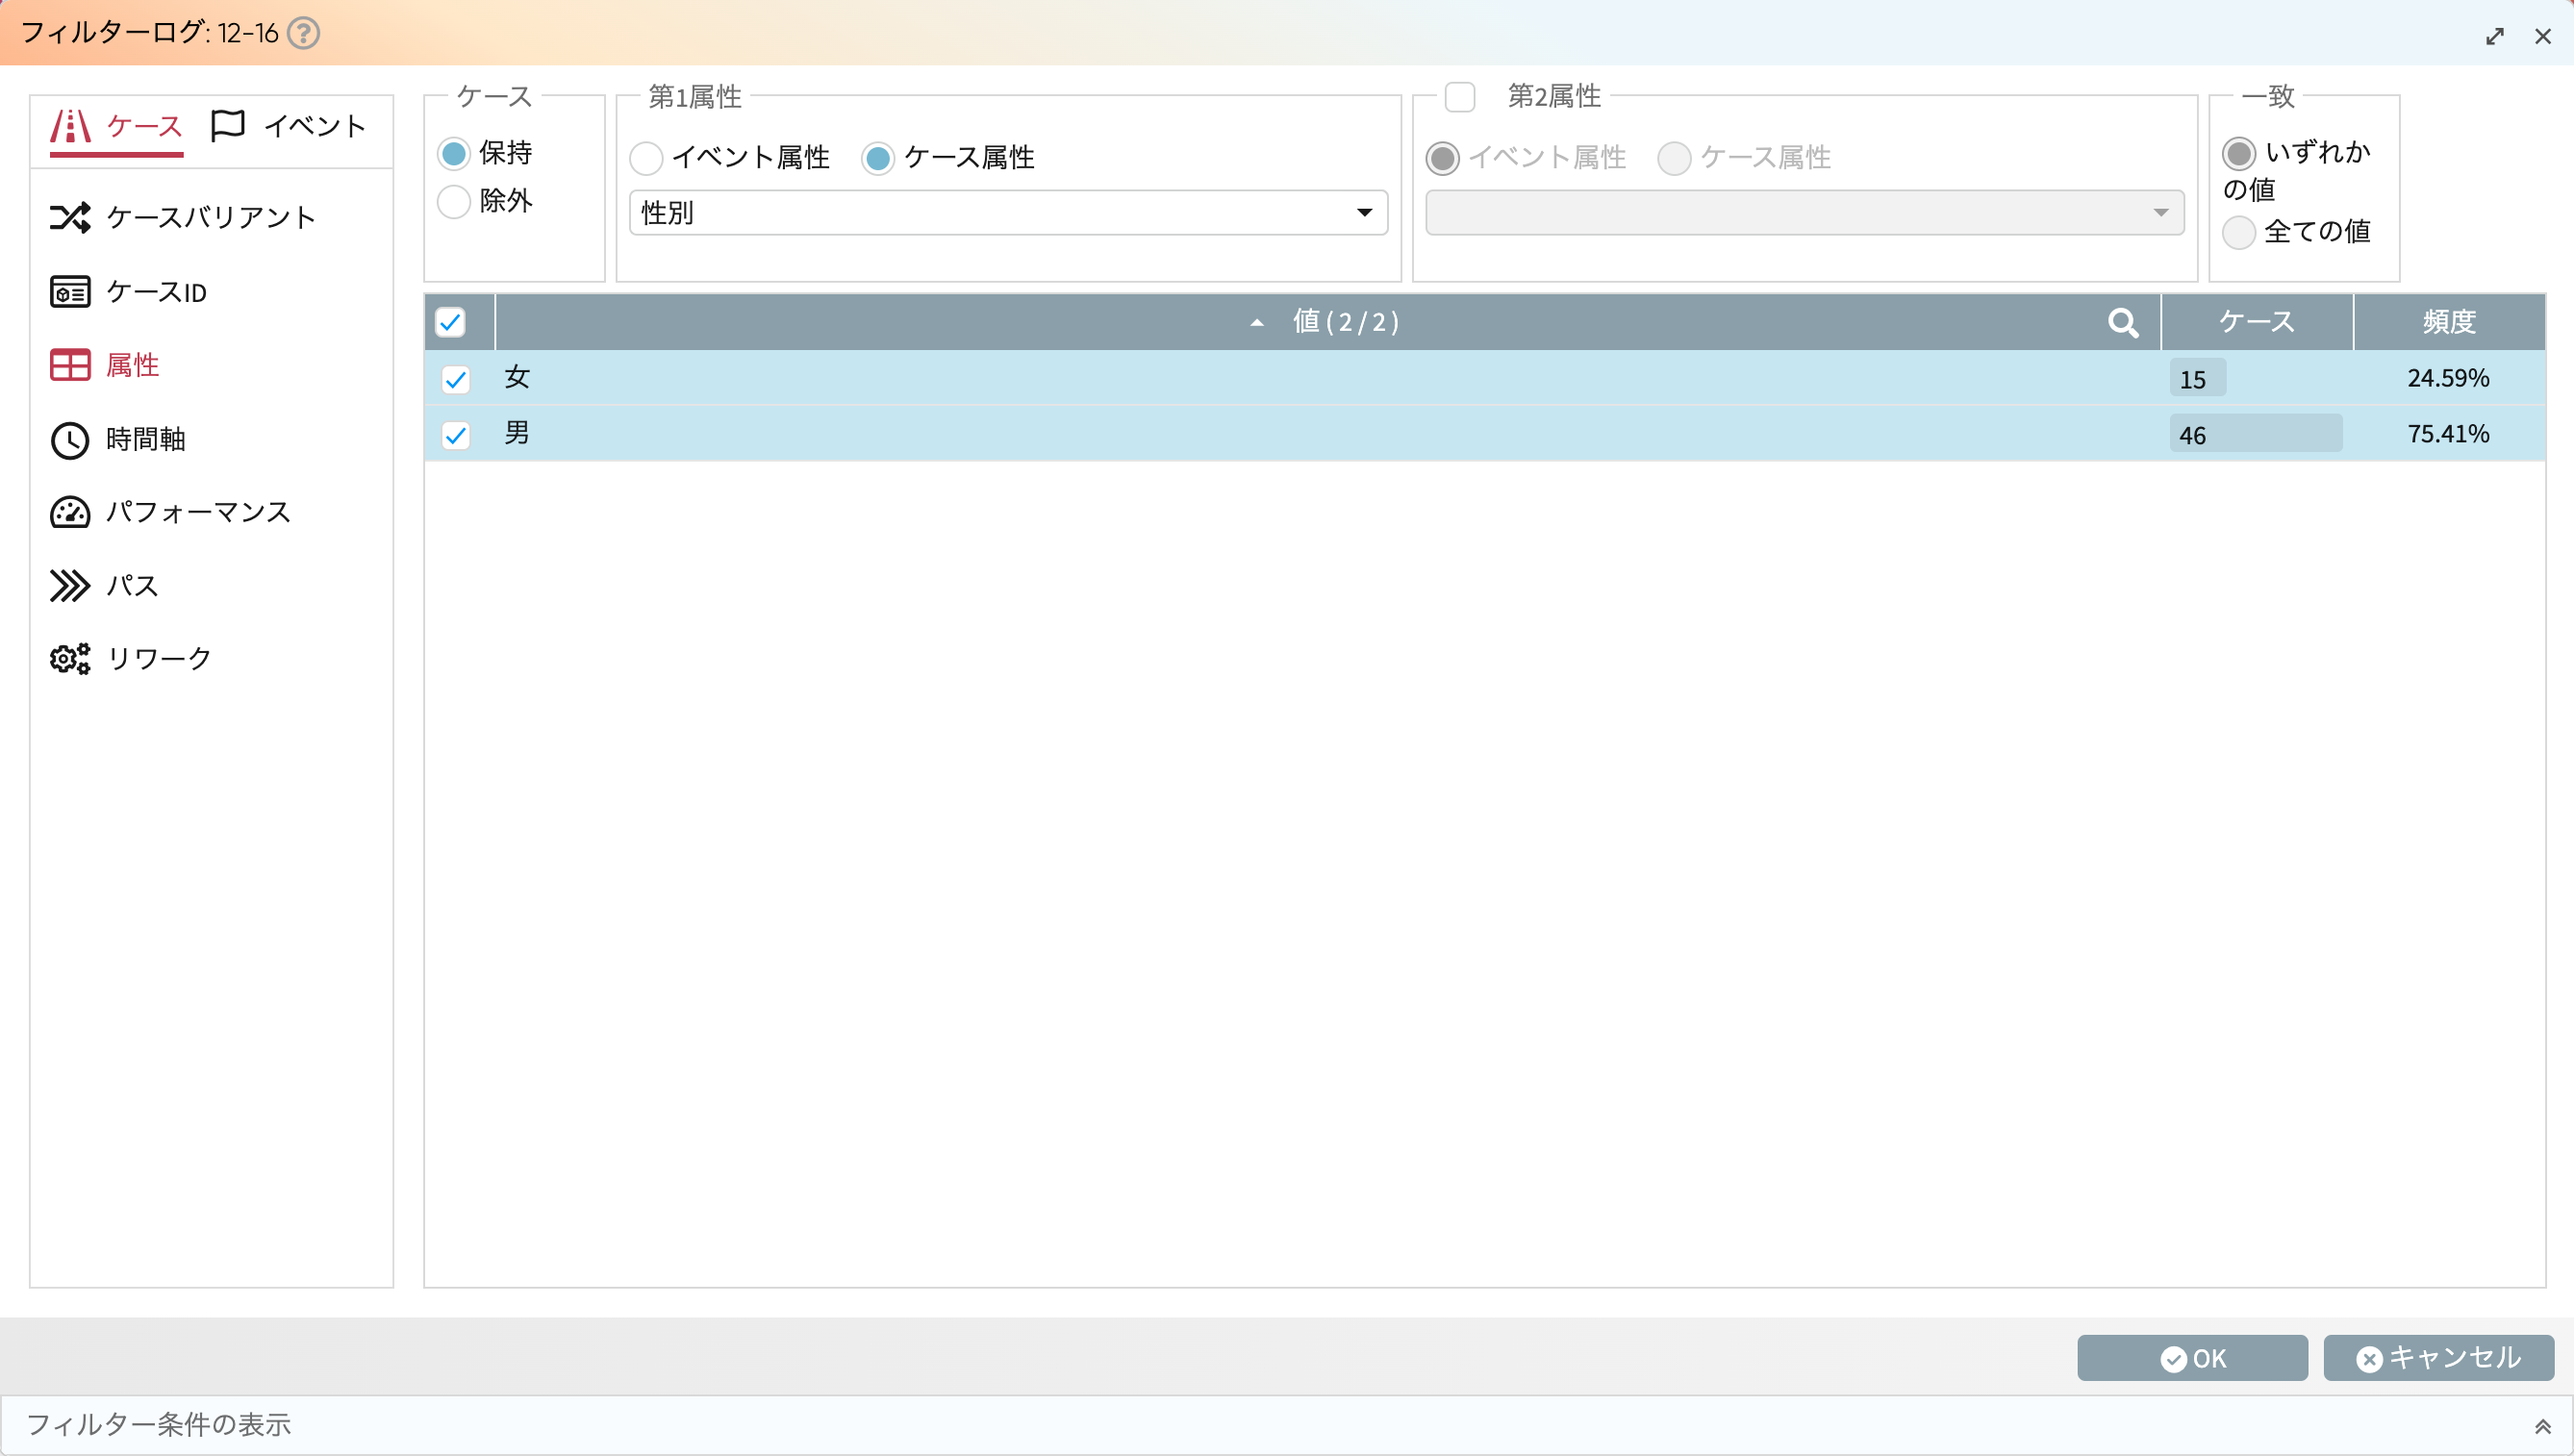
\includegraphics[width=15cm]{1216mw.png}
  \caption{計測日時:12/16 12:00〜13:00,ケース属性の性別フィルターログ選択画面}
  \label{fig:1216mw}
\end{figure}

\begin{figure}[H]
  \centering
  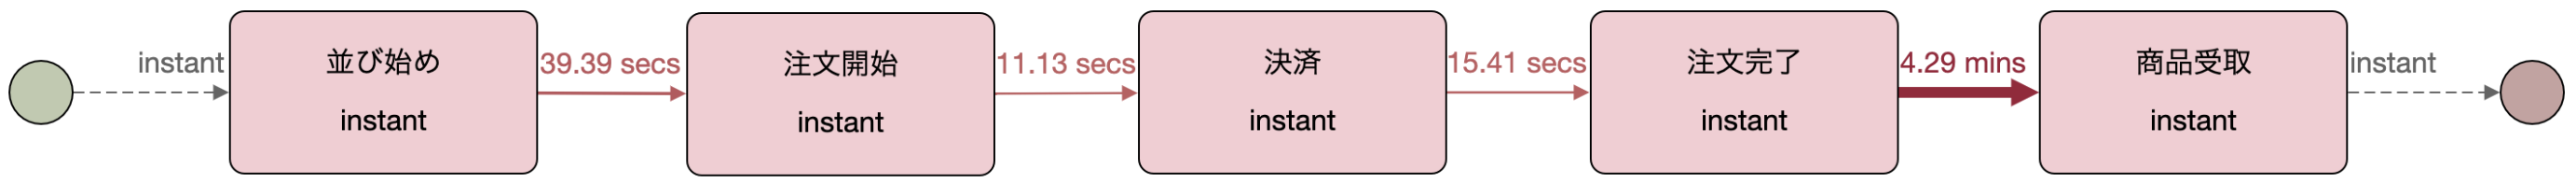
\includegraphics[width=15cm]{man2.png}
  \caption{計測日時:12/16 12:00〜13:00,性別:男,来店数:46人の各計測項目の平均時間}
  \label{fig:man2}
\end{figure}
  
\begin{figure}[H]
  \centering
  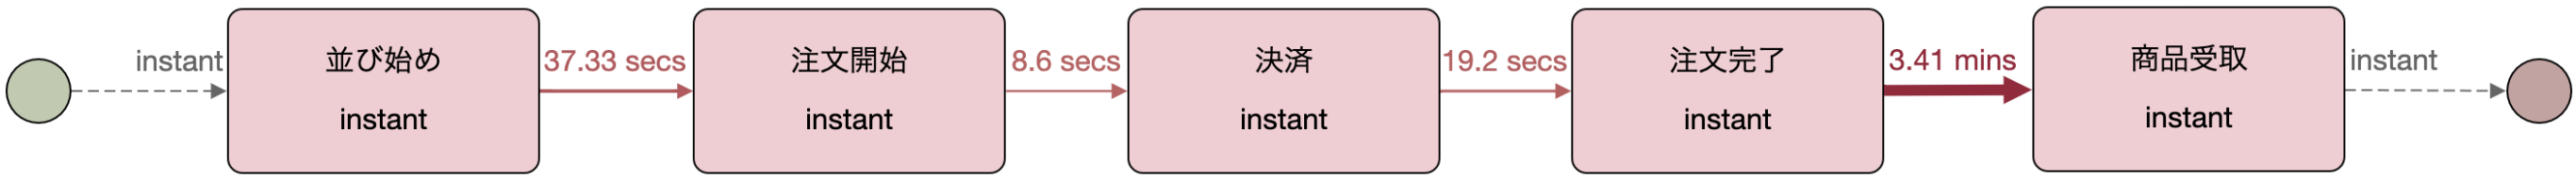
\includegraphics[width=15cm]{woman2.png}
  \caption{計測日時:12/16 12:00〜13:00,性別:女,来店数:15人の各計測項目の平均時間}
  \label{fig:woman2}
\end{figure}


12/16 12:00〜13:00の行列計測データのグループ人数フィルターログ選択画面を図\ref{fig:1216123}に示す。
真ん中より少し上に位置する水色の部分のチェック部分でグループ人数を切り替えて
フィルターログを得ることができる。
グループ人数それぞれの各計測項目の平均時間を
図\ref{fig:1-5b},図\ref{fig:2-5b},図\ref{fig:3-5b},図\ref{fig:4-5b},図\ref{fig:5-5b}に示す。
図\ref{fig:1-5b}〜図\ref{fig:5-5b}は12:00〜13:00の
グループ人数別のデータのプロセスマップであり、左から順に行列に並んだ時間、
注文にかかった時間、決済から注文完了にかかった時間、
商品の受取待ち時間の各平均時間を表している。

\begin{figure}[H]
  \centering
  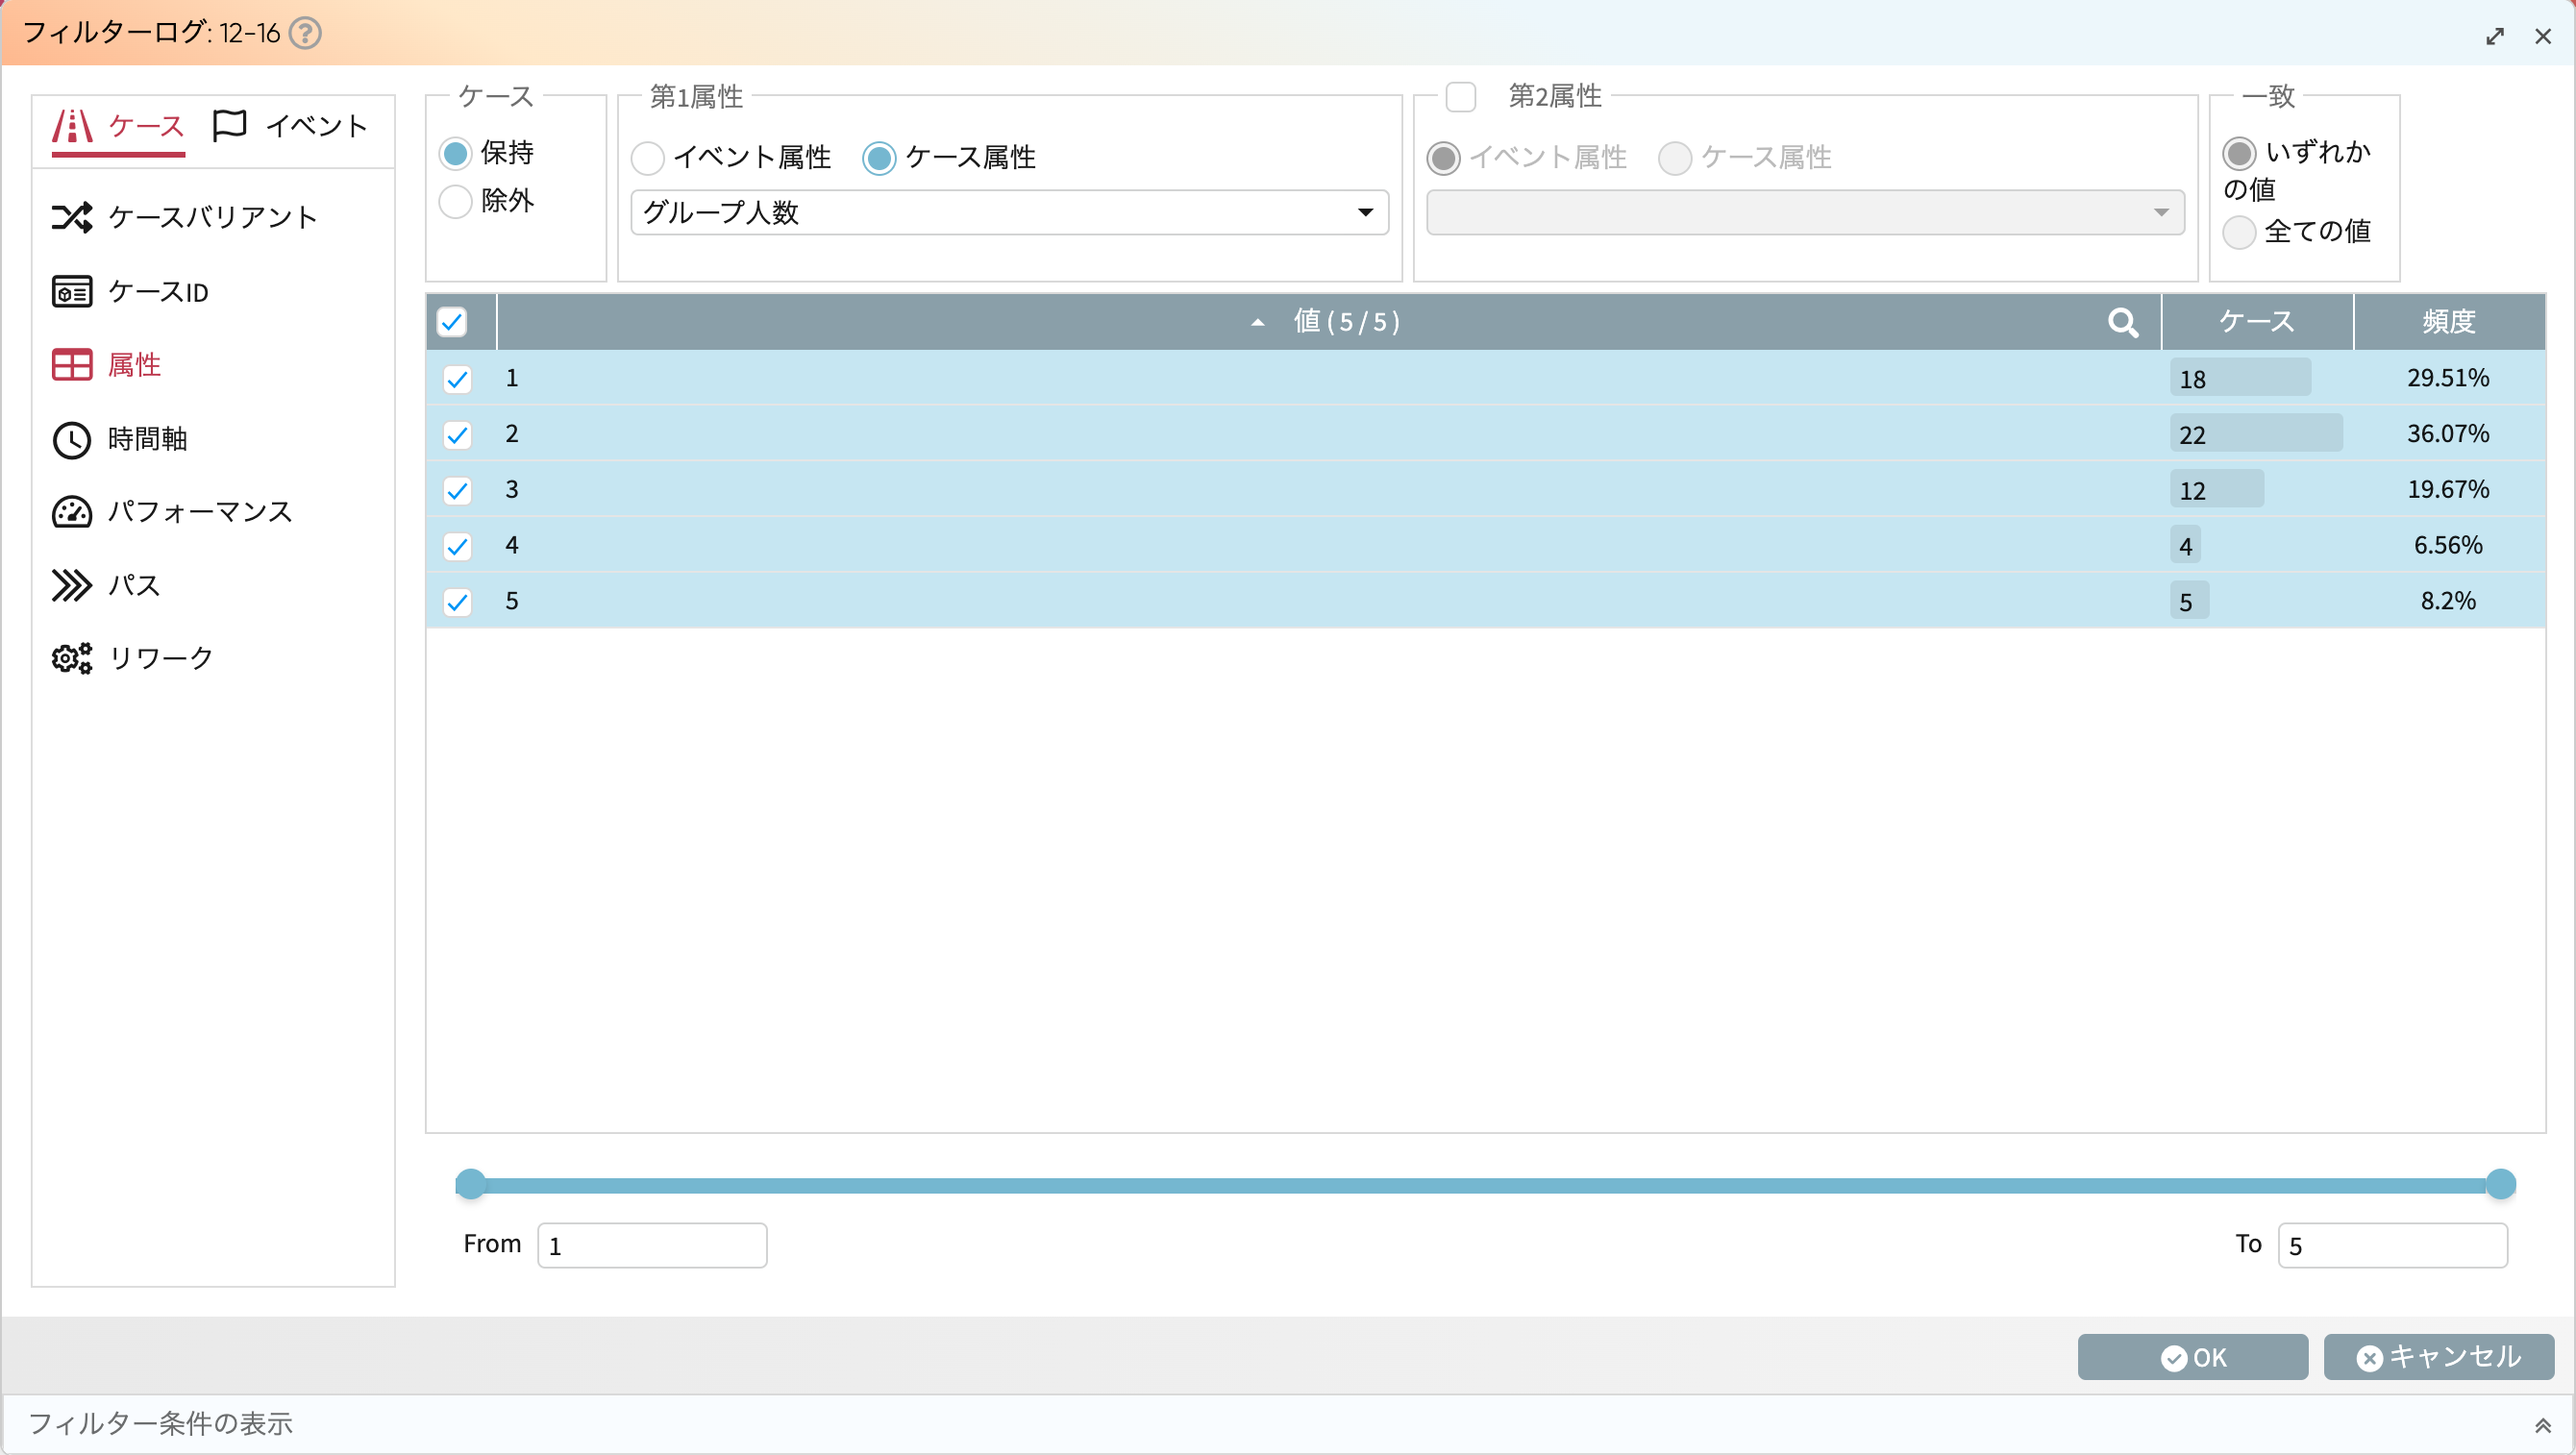
\includegraphics[width=15cm]{1216123.png}
  \caption{計測日時:12/16 12:00〜13:00,ケース属性のグループ人数フィルターログ選択画面}
  \label{fig:1216123}
\end{figure}

\begin{figure}[H]
  \centering
  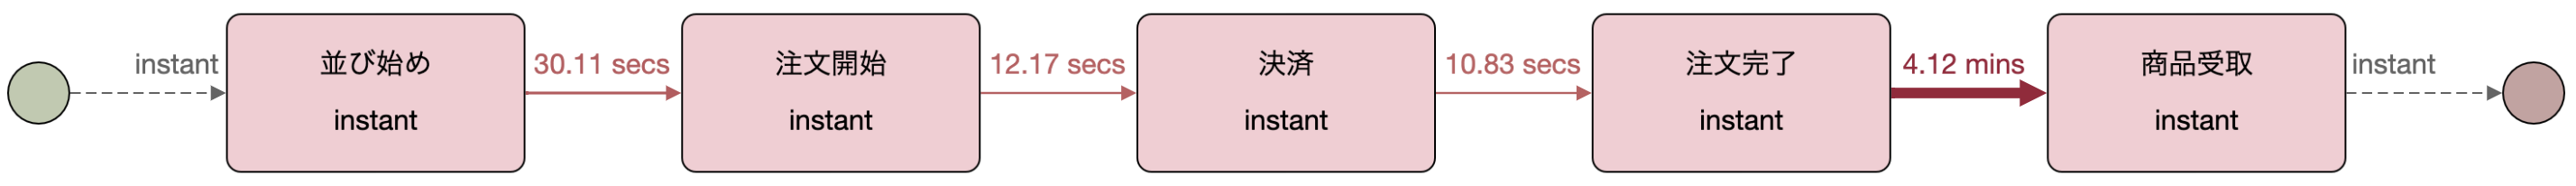
\includegraphics[width=15cm]{1-5b.png}
  \caption{計測日時:12/16 12:00〜13:00,グループ人数:1,来店数:18人の各計測項目の平均時間}
  \label{fig:1-5b}
\end{figure}

\begin{figure}[H]
  \centering
  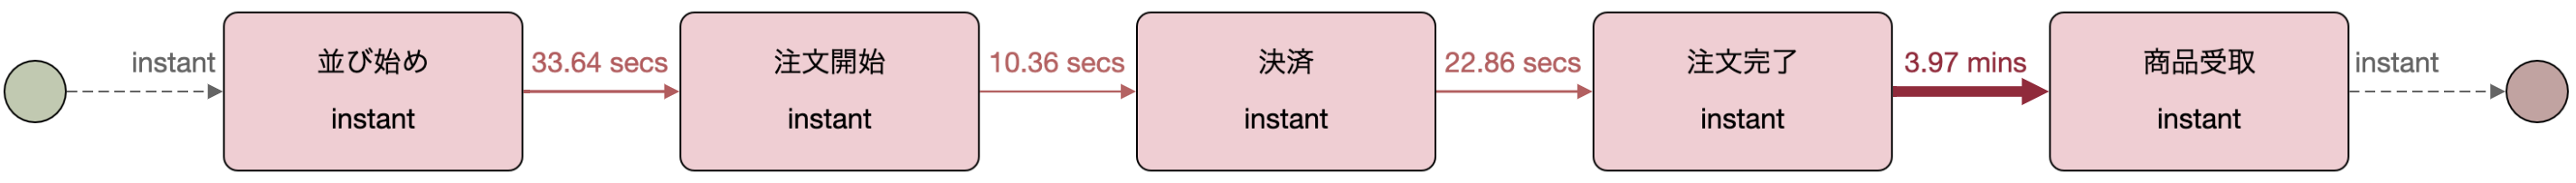
\includegraphics[width=15cm]{2-5b.png}
  \caption{計測日時:12/16 12:00〜13:00,グループ人数:2,来店数:22人の各計測項目の平均時間}
  \label{fig:2-5b}
\end{figure}

\begin{figure}[H]
  \centering
  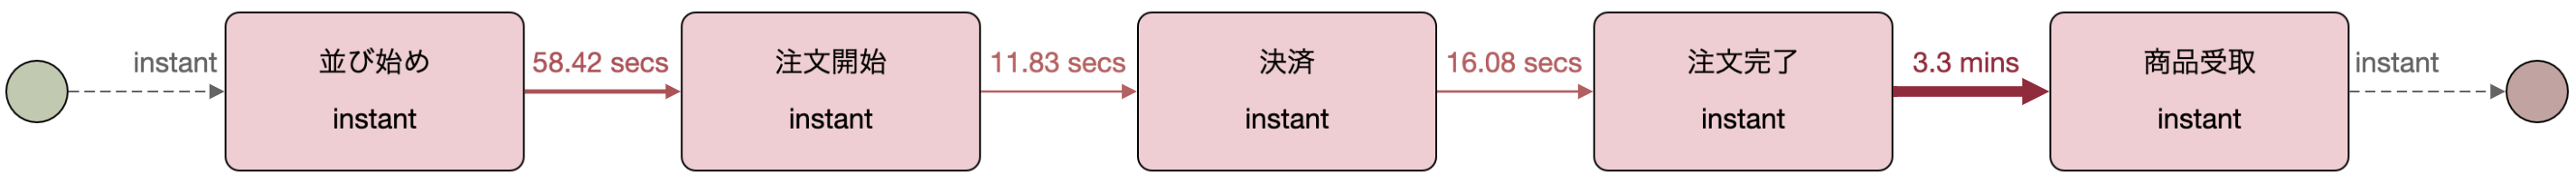
\includegraphics[width=15cm]{3-5b.png}
  \caption{計測日時:12/16 12:00〜13:00,グループ人数:3,来店数:12人の各計測項目の平均時間}
  \label{fig:3-5b}
\end{figure}

\begin{figure}[H]
  \centering
  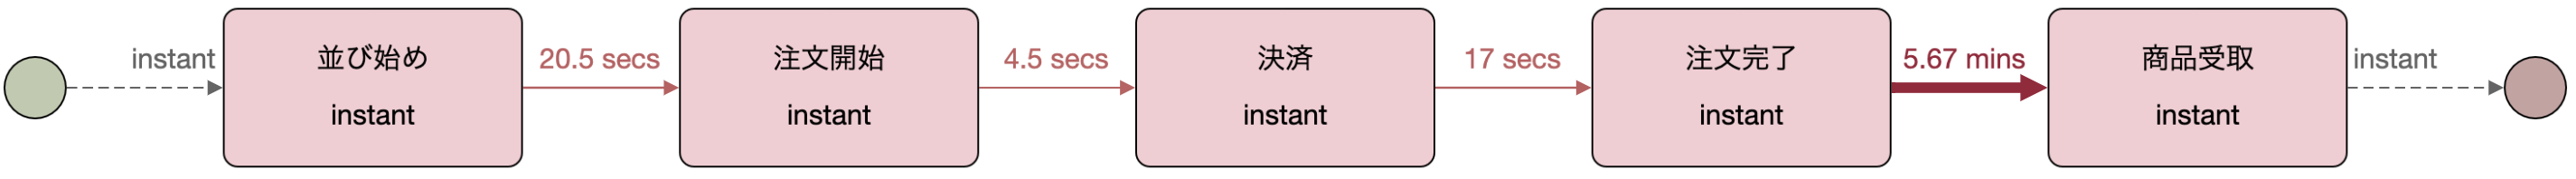
\includegraphics[width=15cm]{4-5b.png}
  \caption{計測日時:12/16 12:00〜13:00,グループ人数:4,来店数:4人の各計測項目の平均時間}
  \label{fig:4-5b}
\end{figure}

\begin{figure}[H]
  \centering
  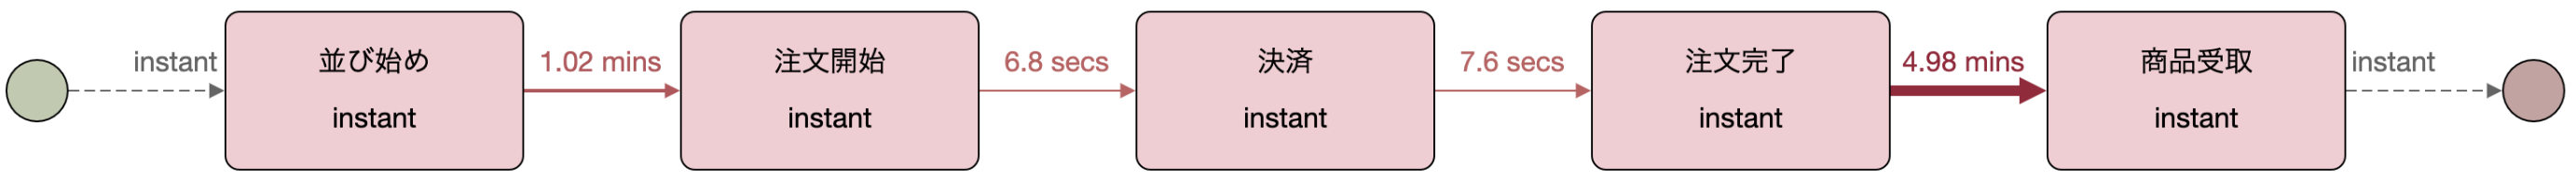
\includegraphics[width=15cm]{5-5b.png}
  \caption{計測日時:12/16 12:00〜13:00,グループ人数:5,来店数:5人の各計測項目の平均時間}
  \label{fig:5-5b}
\end{figure}
%------------------------------------------------------------------





%------------------------------------------------------------------
計測項目を新たに追加して12月に再計測を行ったデータの分析結果を
表\ref{table7},表\ref{table8}に示す。
本研究で計測した行列の計測項目において、客の区分によって変動しうるのは
注文開始から注文完了までと考えられるので、客の区分によっての
注文時間,決済時間の違いを比較する。
行列時間と商品受取待ち時間は客の区分ではなく、客数やお店側に委ねられるので変動しない。

\begin{table}[H]
 \begin{center}
  \caption{12/14に計測したデータの平均時間(小数点第二位四捨五入)}
    \begin{tabular}{|c|c|c|c|c|c|c|} \hline
区分 & 来店数 & 割合 & 行列時間 & 注文時間 & 決済時間 & 商品受取待ち時間 \\ \hline\hline
全体  & 73 & 100\%  & 1分10秒 & 5.6秒 & 14.5秒 & 6分25秒 \\ \hline \hline
男    & 67 & 91.8\% & 1分6秒  & 5.7秒 & 14.6秒 & 6分29秒 \\ \hline
女    & 6  & 8.2\%  & 1分57秒 & 4.5秒 & 13.7秒 & 5分35秒  \\ \hline \hline
1人   & 23 & 31.5\% & 56.4秒  & 5.5秒 & 12.5秒 & 6分14秒 \\ \hline
2人   & 32 & 43.8\% & 1分11秒 & 5.4秒 & 16.8秒 & 6分10秒 \\ \hline
3人   & 18 & 24.7\% & 1分27秒 & 6.2秒 & 12.8秒 & 7分4秒  \\ \hline
 \end{tabular}
 \label{table7}
 \end{center}
\end{table}

表\ref{table7}より、性別の区分を見ると男に比べ女の方が注文時間は1.2秒短く、
決済時間は0.9秒短かった。
グループ人数ごとの区分を1人と比較すると以下のようになる。
\begin{itemize}
\item 2人の方は注文時間は0.1秒短く決済時間は4.3秒長かった。
\item 3人の方は注文時間は0.7秒長く決済時間は0.3秒長かった。
\end{itemize}


\begin{table}[H]
 \begin{center}
  \caption{12/16に計測したデータの平均時間(小数点第二位四捨五入)}
    \begin{tabular}{|c|c|c|c|c|c|c|} \hline
区分 & 来店数 & 割合 & 行列時間 & 注文時間 & 決済時間 & 商品受取待ち時間 \\ \hline \hline
全体 & 61 & 100\%  & 38.9秒 & 10.5秒 & 16.3秒 & 4分4秒 \\ \hline \hline
男   & 46 & 75.4\% & 39.4秒 & 11.1秒 & 15.4秒 & 4分17秒 \\ \hline
女   & 15 & 24.6\% & 37.3秒 & 8.6秒  & 19.2秒 & 3分25秒  \\ \hline \hline
1人  & 18 & 29.5\% & 30.1秒 & 12.1秒 & 10.8秒 & 4分7秒  \\ \hline
2人  & 22 & 36.1\% & 33.6秒 & 10.3秒 & 22.9秒 & 3分58秒 \\ \hline
3人  & 12 & 19.7\% & 58.4秒 & 11.8秒 & 16.1秒 & 3分18秒 \\ \hline
4人  & 4  & 6.6\%  & 20.5秒 & 4.5秒  & 17秒   & 5分40秒 \\ \hline
5人  & 5  & 8.2\%  & 1分    & 6.8秒  & 7.6秒  & 4分58秒 \\ \hline
 \end{tabular}
 \label{table8}
 \end{center}
\end{table}

表\ref{table8}より、性別の区分を見ると男に比べ女の方が注文時間は2.5秒短く、
決済時間は3.8秒長かった。
グループ人数ごとの区分を見ると1人と比較すると以下のようになる。
\begin{itemize}
\item 2人の方は注文時間は1.8秒短く決済時間は12.1秒長かった。
\item 3人の方は注文時間は0.3秒短く決済時間は5.3秒長かった。
\item 4人の方は注文時間は7.6秒短く決済時間は6.2秒長かった。
\item 5人の方は注文時間は5.3秒短く決済時間は3.2秒短かった
\end{itemize}
%------------------------------------------------------------------





\subsection{考察}
5日間の行列計測を行ったが、行列時間や商品受取待ち時間は来店数が増加するに連れ
長くなる傾向がみられた。それを示すデータとして、行列時間は12/16を除いて混雑時の方が待ち時間が長くなっており、商品受取待ち時間は計測日全てにおいて混雑時の方が待ち時間が長くなっていた。

性別やグループ人数別での分析では、ある一定の傾向はみられなかった。
性別の区分における注文時間や決済時間よりもグループの区分における注文時間や決済時間の方が大きく時間差が生じたことが分かった。
これは、友達同士や複数人で券売機を前にすると、同時購入による時間短縮や、券売機前でのメニューの相談による時間遅延が生じたからであると言える。
性別の区分ではあまり差が生じず、グループ人数別ではバラツキが生じやすく一定の傾向はないと考えられる。





\newpage

\section{結論・今後の課題}

店舗販売と併用してモバイルオーダーでのテイクアウト注文を導入した店舗で、
モバイルオーダーでのテイクアウト注文を無制限に受け入れ過ぎたことによって
店舗が混雑し販売に支障をきたす事態や、逆に注文の受け入れ制限をしたことにより
早く注文を処理できた場合に本来受け入れることができた注文分の利益を損失する事態が起きている。
そこで、適切な受け入れ人数を設定するために行列分析を目的とし店舗の行列計測を行い
プロセスマイニングを用いて行列の分析をした。

行列データの収集方法を示し、ExpoGoを用いて近大ラーメンにて行列計測を行った。
4.1章で示したように行列データをプロセスマイニングを用いてフィルタリング等を行い、
プロセスマップを作成し分析することができ行列の特徴を知ることができた。
今後は、モバイルオーダーでのテイクアウト注文を併用する際に店舗での混雑による
支障や利益損失を防ぐために適切な受け入れ人数を設定する必要がある。
また、より多くの行列データを集めて分析することで曜日ごとの特徴などを得ることができると考える。
行列データの収集方法はグループ人数の区分以外はExpoG0を用いて計測できたが、グループ人数は手元の紙にメモをするといった形式だったので、グループ人数の区分もアプリ内でできたら計測もスムーズに行うことができるようになると考えられる。





\newpage

\section{謝辞}
本研究を進めるにあたり御指導、御協力を賜った近畿大学情報学部情報学科森山真光准教授に厚く感謝を申し上げます。
また、行列計測を行う際にご協力いただいた近大をすすらんか、電子商取引研究室の先輩方や同期に深く感謝いたします。


\newpage

\begin{thebibliography}{99}
\bibitem{bibi1} 宇都宮陽一, 奥田隆史. 多段待ち行列モデルを用いた店舗サービスへの it 導入がもたらす影響の分析. 情報処理学会研究報告, 数理モデル化と問題解決 (MPS), 2017.
\bibitem{bibi2} 小池響. 待ち行列理論を用いた事前注文・事前決済 プラットフォームの開発と評価. 卒業論文、近畿大学理工学部情報学科, 2021.
\bibitem{bibi3} 藤井遼. 事前注文・事前決済プラットフォームの開発と導入による待ち行列の評価-事前注文・事前決済プラットフォームの開発-. 卒業論文、近畿大学理工学部情報学科, 2020.
\bibitem{bibi4} 福永光. 待ち行列理論による受け入れ人数の自動調整機能付き事前注文決済システムの開発と評価. 卒業論文、近畿大学理工学部情報学科, 2022.
\bibitem{bibi5} オープンソースではじめるプロセスマイニング. ハートコア株式会社,2022
\end{thebibliography}
\end{document}
